\documentclass{article}
% Use the lineno option to display guide line numbers if required.

% \templatetype{pnasresearcharticle} % Choose template 
% {pnasresearcharticle} = Template for a two-column research article
% {pnasmathematics} %= Template for a one-column mathematics article
% {pnasinvited} %= Template for a PNAS invited submission

\usepackage{authblk}
\usepackage{amsmath,amsfonts,amssymb}
\usepackage[numbers,square,sort&compress]{natbib}
\usepackage[colorlinks=true, allcolors=blue]{hyperref}
\usepackage{graphicx}
\usepackage{booktabs}
\usepackage[margin=1in]{geometry}







% Math
\def\P{\mathbb{P}}
\def\cor{\mathrm{cor}}
\def\Quantile{\mathrm{Quantile}}
\def\logit{\mathrm{logit}}
\def\dist{\mathrm{dist}}
\def\WIS{\mathrm{WIS}}
\def\AUC{\mathrm{AUC}}
\def\CCF{\mathrm{CCF}}
\newcommand{\indicator}[1]{\mathbf{1}\left(#1\right)}

% Figures and tables
\usepackage{xurl}
\usepackage{microtype}
\usepackage{booktabs}
\usepackage{caption}
\usepackage{subcaption}
\usepackage{xcolor}
\newcommand{\attn}[1]{\textcolor{red}{[ATTN: #1]}}

\makeatletter 
\renewcommand\@biblabel[1]{#1} 
\makeatother

% indicators
\newcommand{\chngcli}{CHNG-CLI}
\newcommand{\chngcov}{CHNG-COVID}
\newcommand{\dv}{DV-CLI}
\newcommand{\ar}{AR}
\newcommand{\fb}{CTIS-CLI-in-community}
\newcommand{\gs}{Google-AA}


\title{Can Auxiliary Indicators Improve COVID-19 Forecasting and Hotspot  
  Prediction?} 

% Use letters for affiliations, numbers to show equal authorship (if applicable)
% and to indicate the corresponding author 

% Writing group
\author[a,1]{Daniel J. McDonald}
\author[b,2]{Jacob Bien}
\author[c,2]{Alden Green}
\author[c,d,2]{Addison J. Hu}

% Middle authors
\author[d]{Nat DeFries}
\author[b]{Sangwon Hyun}
\author[c,d]{Natalia L. Oliveira}
\author[e]{James Sharpnack}
\author[f]{Jingjing Tang}
\author[g,h]{Robert Tibshirani}
\author[c]{Val{\'e}rie Ventura}
\author[c,d]{Larry Wasserman}

% Senior authors
\author[c,d]{Ryan J. Tibshirani}

\affil[a]{Department of Statistics, University of British Columbia}
\affil[b]{Department of Data Sciences and Operations, University of Southern
  California} 
\affil[c]{Department of Statistics \& Data Science, Carnegie Mellon University}
\affil[d]{Machine Learning Department, Carnegie Mellon University}
\affil[e]{Department of Statistics, University of California, Davis}
\affil[f]{Computational Biology Department, Carnegie Mellon University}
\affil[g]{Department of Statistics, Stanford University}
\affil[h]{Department of Biomedical Data Science, Stanford University}




% Please add a significance statement to explain the relevance of your work
% \significancestatement{Forecasting is a critical element in the public health
%   response to any fast-moving epidemic or pandemic.  Predicting the future
%   spread of some disease process, based on disease activity in the recent
%   past---say, using what is known as autoregressive modeling in the time series
%   literature---is a basic and widely-used method.  In this paper we study
%   whether including auxiliary indicators as additional features in such an
%   autoregressive model can be useful in COVID-19 case forecasting and hotspot
%   prediction.  We find that indicators based on de-identified medical insurance 
%   claims, self-reported symptoms through online surveys, and COVID-related
%   internet search activity all provide a nontrivial boost in accuracy, though
%   their utility generally depends the pandemic's local dynamics (upswing,
%   downswing, or flat period) at prediction time.
% }

% At least three keywords are required at submission. Please provide three to
% five keywords, separated by the pipe symbol. 




\begin{document}

\maketitle

\begin{abstract}
  Reliable, short-term forecasts of traditional public health reporting streams
  (such as cases, hospitalizations, and deaths) are a key ingredient in
  effective public health decision-making during a pandemic. Since April 2020,
  our research group has worked with data partners to collect, curate, and make
  publicly available numerous real-time COVID-19 indicators, providing multiple
  views of pandemic activity.  This paper studies the utility of these
  indicators from a forecasting perspective. We focus on five indicators,
  derived from medical insurance claims data, web search queries, and online
  survey responses. For each indicator, we ask whether its inclusion in a simple
  model leads to improved predictive accuracy relative to a similar model
  excluding it. We consider both probabilistic forecasting of confirmed COVID-19
  case rates and binary prediction of case ``hotspots''.  Since the values of 
  indicators (and case rates) are commonly revised over time, we take special
  care to ensure that the data provided to a forecaster is the version that
  would have been available at the time the forecast was made.   
  % We demonstrate how less careful backtesting can lead to misleading
  % retrospective evaluations.   
  Our  analysis shows that consistent but modest gains in predictive accuracy 
  are obtained by using these indicators, and furthermore, these gains are
  related to periods in which the auxiliary indicators behave as ``leading
  indicators'' of case rates.

  {\bf Keywords:} COVID-19 $|$ forecasting $|$ hotspot prediction $|$ time series
    $|$ digital surveillance
\end{abstract}

\footnotetext[1]{To whom correspondence should be
  addressed. E-mail: \href{mailto:daniel@stat.ubc.ca}{daniel@stat.ubc.ca}} 
\footnotetext[2]{J.B., A.G., and A.J.H. contributed equally to 
  this work.}

\clearpage


Tracking and forecasting indicators from public health reporting
streams---such as confirmed cases and deaths in the COVID-19 pandemic---is
crucial for understanding disease spread, formulating public policy responses,
and anticipating future public health resource needs.  In a companion paper, we
describe our research group's (Delphi's) efforts in curating and maintaining a 
database of real-time indicators that track COVID-19 activity and other relevant
phenomena. The signals (a term we use synonomously with ``indicators'') in this
database are accessible through the COVIDcast API \cite{CovidcastAPI}, with
associated R \cite{CovidcastR} and Python \cite{CovidcastPy} packages for
convenient data fetching and processing tools. In the current paper, we aim to
quantify the utility provided by a core set of these indicators for two
fundamental prediction tasks: probabilistic forecasting of COVID-19 case 
rates and prediction of future COVID-19 case hotspots (defined by the event that
a relative increase in COVID-19 cases exceeds a certain threshold). 

 At the outset, we should be clear that our intent in this paper is \textit{not}
to provide an authoritative take on cutting-edge COVID-19 forecasting methods.
Instead, our purpose here is to provide a rigorous, quantitative assessment of
the utility that several auxiliary indicators---such as those derived from
internet surveys or medical insurance claims---provide in tasks that involve
predicting future trends in confirmed COVID-19 cases. To assess such utility in
as simple terms as possible, we center our study in the framework of a basic
autoregressive model (in which COVID cases in the near future are predicted from  
a linear combination of COVID cases in the near past), and ask whether the 
inclusion of an auxiliary indicator as an additional feature in such a model
improves its predictions. 

While forecasting carries a rich literature that offers a wide range of
techniques, see e.g., \cite{Hyndman:2018}, we purposely constrain ourselves to
very simple models, avoiding common enhancements such as order selection,
correction of outliers/anomalies in the data, and inclusion of regularization or
nonlinearities. That said, analyses of forecasts submitted to the COVID-19
Forecast Hub \cite{ForecastHub} by a large community of modelers have shown that
simple, robust models have consistently been among the best-performing over the
pandemic \cite{Cramer:2021}, including time series models similar to those we
consider in what follows.   

In our companion paper, we analyze correlations between various indicators and   
COVID case rates. These correlations are natural summaries of the
contemporaneous association between an indicator and COVID cases, but they fall 
short of delivering a satisfactory answer to the question that motivates the
current article: is the information contained in an indicator demonstrably
useful for the prediction tasks we care about? For such a question, lagged
correlations (e.g., measuring the correlation between an indicator and COVID
case rates several days in the future) move us in the right direction, but still
do not move us all the way there. The question about \textit{utility for 
  prediction} is focused on a much higher standard than simply asking 
about correlations; to be useful in forecast or hotspot models, an indicator
must provide relevant information that is not otherwise contained in past values
of the case rate series itself. We will assess this in the most direct way
possible: by inspecting the difference in predictive performance of simple
autoregressive models trained with and without access to past values of a
particular indicator.   

There is another, more subtle issue in evaluating predictive utility that 
deserves explicit mention, as it will play a key role in our analysis.
Signals computed from surveillance streams will often be subject to  
latency and/or revision. For example, a signal based on aggregated medical
insurance claims may be available after just a few days, but it can then be
substantially revised over the next several weeks as additional claims are
submitted and/or processed late. Correlations between such a signal and case
rates calculated ``after the fact'' (i.e., computed retrospectively, using the
finalized values of this signal) will not deliver an honest answer to the    
question of whether this signal would have been useful in real time. Instead,
we build predictive models using only the data that would have been available
\textit{as of} the prediction date, and compare the ensuing predictions in terms 
of accuracy. To do so, we leverage Delphi's \texttt{evalcast} R package 
\cite{EvalcastR}, which plugs into the COVIDcast API's data versioning system,  
and facilitates honest backtesting. 

Finally, it is worth noting that examining the importance of additional features
for prediction is a core question in inferential statistics and econometrics,
with work dating back to at least \cite{Granger:1969}. Still today, drawing
rigorous inference based on predictions, without (or with lean) assumptions, is
an active field of research from both the applied and theoretical angles;
see, e.g., \cite{Diebold:2002, McCraken:2007, Diebold:2015, Stokes:2017,
  Lei:2018, Rinaldo:2019, Williamsom:2020, Zhang:2020, Dai:2021, Fryer:2021}.
Our take on this problem is in line with much of this literature; however, in
order to avoid making any explicit assumptions, we do not attempt to make formal 
significance statements, and instead, broadly examine the stability of our
conclusions with respect to numerous modes of analysis.   

\section{Methods}

\subsection{Signals and Locations}

We consider prediction of future COVID-19 case rates or case hotspots (to be
defined precisely shortly).  By case rate, we mean the case count per 100,000
people (the standard in epidemiology).  We use reported case data aggregated by 
JHU CSSE \cite{Dong:2020}, which, like the auxiliary indicators that we use to
supplement the basic autoregressive models, is accessible through the COVIDcast
API \cite{CovidcastAPI}. 

The indicators we focus on provide information not generally available from
standard public health reporting. Among the many auxiliary indicators collected
in the API, we study the following five:  
\begin{itemize}
\item Change Healthcare COVID-like illness (CHNG-CLI): The percentage of
  outpatient visits that are primarily about COVID-related symptoms, based on
  de-identified Change Healthcare claims data.
\item Change Healthcare COVID (CHNG-COVID): The percentage of outpatient visits
  with confirmed COVID-19, based on the same claims data.
\item COVID Trends and Impact Survey COVID-like illness in the community
  (CTIS-CLI-in-community): The estimated percentage of the population who know
  someone in their local community who is sick, based on Delphi's COVID Trends
  and Impact Survey, in partnership with Facebook.
\item Doctor Visits COVID-like illness (DV-CLI): The same as CHNG-CLI, but
  computed based on de-identified medical insurance claims from other health
  systems partners.  
\item Google search trends for anosmia and ageusia (Google-AA): A measure of  
  Google search volume for queries that relate to anosmia or ageusia (loss of
  smell or taste), based on Google's COVID-19 Search Trends data set.  
\end{itemize}
In short, we choose these indicators because, conceptually speaking, they
measure aspects of an individual's disease progression that would plausibly
precede the occurence of (at worst, co-occur  with) the report of a positive
COVID-19 test, through standard public health reporting streams.

For more details on the five indicators (including how these are precisely
computed from the underlying data streams) we refer to
\url{https://cmu-delphi.github.io/delphi-epidata/api/covidcast_signals.html},
which documents all of the signals in the COVIDcast API, and our companion paper
on the API and database. For CTIS in particular, we refer to our companion paper
on this survey. For the Google COVID-19 Search Trends data set, see
\cite{GoogleSymptoms}; see also \cite{Klopfen:2020, Vaira:2020} for a 
justification of the relevance of anosmia or ageusia to COVID-19 infection. 

As for geographic resolution, we consider the prediction of COVID-19 case rates
and hotspots aggregated at the level of an individual \textit{hospital referral
  region} (HRR). HRRs correspond to groups of counties in the United States
within the same hospital referral system. The Dartmouth Atlas of Healthcare 
Policy~\cite{DartmouthHRR}, defines these 306 regions based on a number of
characteristics. They are contiguous regions such that most of the hospital
services for the underlying population are performed by hospitals within the
region. Each HRR also contains at least one city where major procedures
(cardiovascular or neurological) are performed. The smallest HRR has a
population of about 125,000. While some are quite large (such as the one
containing Los Angeles, which has more than 10 million people), generally HRRs  
are much more homogenous in size than the (approximately) 3200 counties,  
and they serve as a nice middle ground in between counties and states.  

HRRs, by their definition, would be most relevant for forecasting hospital
demand.  We have chosen to focus on cases (forecasting and predicting
hotspots) at the HRR level because the indicators considered should be more 
useful in predicting case activity rather than hospital demand, as the former is  
intuitively more contemporaneous to the events that are measured by
the given five indicators. Predicting case rates (and hotspots) at the HRR level
is still a reasonable goal in its own right; and moreover, it could be used to
feed predicted case information into downstream hospitalization models.

\subsection{Vintage Training Data}

In this paper, all models are fit with ``vintage'' training data. This means
that for a given prediction date, say, September 28, 2020, we train models 
using data that would have been available to us \textit{as of}
September 28 (imagine that we can ``rewind'' the clock to September 28 and query
the COVIDcast API to get the latest data it would have had available at that
point in time.)  This is possible because of the COVIDcast API's comprehensive
data versioning system (described in more detail in our companion paper).  We
also use the \texttt{evalcast} R package \cite{EvalcastR}, which streamlines the 
process of training arbitrary prediction models over a sequence of prediction
dates, by constructing the proper sequence of vintage training data sets.   

\begin{figure}[tb!]
  \centering
  \includegraphics[width=.5\linewidth]{fig/revisions.pdf}
  % RJT: Ensuring we start with a "declarative title" :) 
  % https://www.internationalscienceediting.com/how-to-write-a-figure-caption/
  \caption{Revision behavior for two indicators in the HRR containing Charlotte, 
    North Carolina.  Each colored line corresponds to the data as reported on a
    particular date (\textit{as of} dates varying from September 28 through
    October 19). The left panel shows the DV-CLI signal, which was regularly
    revised throughout the period, though the effects fade as we look further
    back in time. In contrast, the right panel shows case rates reported by JHU
    CSSE (smoothed with a 7-day trailing average), which remain ``as reported''
    on September 28, with a spike towards the end of this period, until a major 
    correction is made on October 19, which brings this down and affects all
    prior data as well.}  
  \label{fig:vintage}
\end{figure}

Vintage training data means different things, in practice, for different
signals. The three signals based on medical claims, CHNG-CLI, CHNG-COVID, and
DV-CLI, are typically 3-5 days latent, and subject to a considerable but
regular degree of revision or ``backfill'' after their initial publication date.
The survey-based signal, CTIS-CLI-in-community, is 2 days latent, and rarely
undergoes any revision at all.  The target variable itself, reported COVID-19
case rates, is 1 day latent, and exhibits frequent, unpredictable revisions
after intial publication.  Compared to the pattern of revisions in the medical 
claims signals, which are much more systematic in nature, revisions in case
reports can be highly erratic. Big spikes or other anomalies can occur in the
data as reporting backlogs are cleared, changes in case definitions are made,
etc. Groups like JHU CSSE then work tirelessly to correct such anomalies after
first publication (e.g., they will attempt to back-distribute a spike when a
reporting backlog is cleared, by working with a local authority to figure out
how this should best be done), which can result in very nontrivial revisions.
See Figure~\ref{fig:vintage} for an example. 

Lastly, our treatment of the Google-AA signal is different from the rest.
Because Google's team did not start publishing this signal until early
September, 2020, we do not have true vintage data before then.  Furthermore, the
latency of the signal was always at least one week through 2020.  However, this
signal is never revised after initial publication (confirmed via personal
communication with the Google team that produces this signal) and furthermore
the latency of the signal is not an unavoidable property of the data type, so we
simply use finalized signal values, with zero latency, in our analysis.   

\subsection{Analysis Tasks}

\begin{table*}[t]
\centering
\caption{Summary of forecasting and hotspot prediction tasks considered in
  this paper.}
\begin{tabular}{l p{2.25in} p{2.25in}}
  \toprule
  & \textbf{Forecasting} & \textbf{Hotspot prediction} \\
  \midrule
  Response variable & $Y_{\ell,t}$ (7-day trailing average of COVID-19 case 
incidence rates, per location $\ell$ and time $t$) & $Z_{\ell,t} =
\indicator{Y_{\ell,t} \geq 1.25 \cdot Y_{\ell,t-7}}$ (indicator that 
$Y_{\ell,t}$ grows by more than 25\% relative to the preceding week) \\ 
  Geographic resolution & Hospital referral region (HRR) & Hospital referral
region (HRR) \\ 
  Forecast period & June 9--December 31, 2020 & June 16--December 31, 2020 \\  
  Model type & Quantile regression & Logistic regression \\
  Evaluation metric & Weighted interval score (WIS) & Area under curve (AUC) \\
  \bottomrule
\end{tabular}
\label{tab:analysis_tasks}
\end{table*}

To fix notation, let $Y_{\ell,t}$ denote the 7-day trailing average of COVID-19
case incidence rates in location (HRR) $\ell$ and at time (day) $t$.  To be
clear, this is the number of new daily reported cases per 100,000
people, averaged over the 7-day period $t-6, \ldots, t$. The first task we
consider---\textit{forecasting}---is to predict $Y_{\ell,t+a}$ for each
``ahead'' value $a=7,\ldots,21$.  The second task---\textit{hotspot
  prediction}---is to predict a binary variable defined in terms of the relative
change of $Y_{\ell,t+a}$ (relative to its value one week prior,
$Y_{\ell,t+a-7}$), again for each $a=7,\ldots,21$.   

Why do we define the response variables via 7-day averaging? The short answer 
is robustness: averaging stabilizes the case time series, and accounts for 
uninteresting artifacts like day-of-the-week effects in the series.  Note that
we can also equivalently view this (equivalent up to a constant factor) as
predicting the HRR-level case incidence rate \textit{summed} over some 7-day
period in the future, and predicting a binary variable derived from this.     

In what follows, we cover more details on our two analysis
tasks. Table~\ref{tab:analysis_tasks} presents a summary.   

\paragraph{Dynamic Re-Training}

For each prediction date $t$, we use a 21-day trailing window of data to train
our forecast or hotspot prediction models (so, e.g., the trained models will
differ from those at prediction date $t-1$).  This is done to account for
(potential) nonstationarity.  For simplicity, the forecasting and hotspot
prediction models are always trained on data across all HRRs (i.e., the
coefficients in the models do not account for location-specific effects).   

\paragraph{Prediction Period}

In our analysis, we let the prediction date $t$ run over each day in between
early/mid June and December 31, 2020.  The precise start date differs for 
forecasting and hotspots prediction; for each task it was chosen to be the
earliest date at which the data needed to train all models was available, which
ends up being (per our setup, with 21 days of training data and lagged values 
of signals for features, as we will detail shortly) June 9, 2020 for
forecasting, and June 16, 2020 for hotspot prediction. (The bottleneck here is
the CTIS-CLI-in-community signal, which does not exist before early April 2020,
when the survey was first launched). The end date was chosen again with a 
consideration to align both tasks as best as possible, and because few hotspots
exist post December 31, 2020, due to the general and gradual decline of the
pandemic in 2021.

\paragraph{Forecasting Models}

Recall $Y_{\ell,t}$ denotes the 7-day trailing average of COVID-19 case
incidence rates in location $\ell$ and at time $t$.  Separately for each
$a=7,\ldots,21$, to predict $Y_{\ell,t+a}$ for ahead value $a$, we consider a
simple probabilistic forecasting model of the form:     
\begin{equation}
\label{eq:forecast_ar}
\Quantile_\tau(Y_{\ell,t+a} \ | \ Y_{\ell,s},\ s \leq t)   
= \alpha^{a,\tau} + \sum_{j=0}^2 \beta^{a,\tau}_j Y_{\ell,t-7j}.  
\end{equation}
This model uses current case rates, and the case rates 7 and 14 days ago, in
order to predict (the quantiles of) case rates in the future.  We consider a
total of 7 quantile levels (chosen in accordance with the county-level quantile
levels suggested by the COVID-19 Forecast Hub),      
\begin{equation}
\label{eq:quantile_levels}
\tau \in \{0.025,\ 0.1,\ 0.25,\ 0.5,\ 0.75,\ 0.9,\ 0.975 \}.
\end{equation}
We fit \eqref{eq:forecast_ar} using \textit{quantile regression}
\cite{Koenker:1978, Koenker:2005, Koenker:2006} separately for each $\tau$, 
using data from all 306 HRRs, and within each HRR, using the most recent 21 days
of training data.  This gives us 6,426 training samples for each quantile 
regression problem.    

In addition to this pure autoregressive model, we also consider five
probabilistic forecasting models of the form:  
\begin{equation}
\label{eq:forecast_ar_x}
\Quantile_\tau(Y_{\ell,t+a} \ | \ Y_{\ell,s},\ X_{\ell,s},\ s \leq t) 
= \alpha^{a,\tau} + \sum_{j=0}^2 \beta^{a,\tau}_j Y_{\ell,t-7j} + 
\sum_{j=0}^2 \gamma^{a,\tau}_j X_{\ell,t-7j},
\end{equation}
where $X_{\ell,t}$ denotes any one of the five auxiliary indicators---CHNG-CLI, 
CHNG-COVID, CTIS-CLI-in-community, DV-CLI, or Google-AA---at location $\ell$ and
time $t$. Note that we apply the same lags (current value, along with the values
7 and 14 days ago) for the auxiliary indicators as we do for the case
rates. Training then proceeds just as before: we use the same 7 quantile levels
in \eqref{eq:quantile_levels}, and fit quantile regression separately for each 
level $\tau$, using data from all 306 HRRs and a trailing window of 21 days of
training data.

At prediction time, in order to avoid crossing violations (that is, for two
levels $\tau' > \tau$, the predicted quantile at level $\tau$ exceeds the
predicted quantile at level $\tau'$), we apply a simple post-hoc sorting.  See
Figure~\ref{fig:trajectory} for an example forecast. 

\begin{figure}[t]
  \centering
\includegraphics[width=.5\columnwidth]{fig/trajectory.pdf}
\caption{Forecast for the HRR containing New York City from an autoregressive
  model made on October 15 (vertical line).  The fan displays 50\%, 80\% and
  95\% intervals while the orange curve shows the median forecast. The black
  curve shows ``finalized'' data, as reported in May 2021.}   
\label{fig:trajectory}
\end{figure}

\paragraph{Hotspot Prediction Models}

Define the binary indicator:
$$
Z_{\ell,t} = \indicator{Y^\Delta_{\ell,t} \geq 0.25},
$$
where we use the notation \smash{$Y^\Delta_{\ell,t} = (Y_{\ell,t} - Y_{\ell,
    t-7})/(Y_{\ell,t-7})$}. In other words, $Z_{\ell,t}=1$ if the number of
newly reported cases over the past 7 days has increased by at least 25\%
compared to the preceding week.  When this occurs, we say location $\ell$ is a
\textit{hotspot} at time $t$.  Empirically, this rule labels about 27\% of
location-time pairs as hotspots, during the prediction period (June 16--December
31, 2020).   

We treat hotspot prediction as a binary classification problem and use a setup 
altogether quite similar to the forecasting setup described previously.
Separately for each $a=7,\ldots,21$, to predict $Z_{\ell,t+a}$, we consider a
simple logistic model:
\begin{equation}
\label{eq:hotspot_ar}
\logit \big( \P(Z_{\ell,t+a} = 1 \ | \ Y_{\ell,s},\ s \leq t) \big) 
= \alpha^{a,\tau} + \sum_{j=0}^2 \beta^{a,\tau}_j Y^\Delta_{\ell,t-7j},
\end{equation}
where $\logit(p) = \log(p/(1-p))$, the log-odds of $p$.

In addition to this pure autoregressive model, we also consider five
logistic models of the form:  
\begin{equation}
\label{eq:hotspot_ar_x}
\logit \big( \P(Z_{\ell,t+a} = 1 \ | \ Y_{\ell,s},\ X_{\ell,s},\ s \leq t) \big)
=  \alpha^{a,\tau} + \sum_{j=0}^2 \beta^{a,\tau}_j Y^\Delta_{\ell,t-7j} +  
\sum_{j=0}^2 \gamma^{a,\tau}_j X^\Delta_{\ell,t-7j},
\end{equation}
where we use \smash{$X^\Delta_{\ell,t} = (X_{\ell,t} - X_{\ell,
    t-7})/(X_{\ell,t-7})$}, and again $X_{\ell,t}$ stands for any of the five  
auxiliary indicators at location $\ell$ and time $t$.  We fit the above models,
\eqref{eq:hotspot_ar}, \eqref{eq:hotspot_ar_x}, using logistic regression,   
pooling all 306 HRRs and using a 21-day trailing window for the training data.   

An important detail is that in hotspot prediction we remove all data from
training and evaluation where, on average, fewer than 30 cases (this refers to a
count, not a rate) are observed over the preceding 7 days. This avoids having to
make arbitrary calls for a hotspot (or lack thereof) based on small counts.   

\subsection{Evaluation Metrics}

For forecasting, we evaluate the probabilistic forecasts produced by the
quantile models in \eqref{eq:forecast_ar} and \eqref{eq:forecast_ar_x} using 
\textit{weighted interval score} (WIS), a quantile-based scoring rule; see e.g.,
\cite{Gneiting:2007}.  WIS is a proper score, which means that its expectation 
is minimized by the population quantiles of the target variable.  The use of WIS
in COVID-19 forecast scoring is discussed in \cite{Bracher:2021}; WIS is also
the main evaluation metric used in the COVID-19 Forecast Hub.

WIS is typically defined for quantile-based forecasts where the quantile levels
are symmetric around 0.5.  This is the case for our choice in
\eqref{eq:quantile_levels}.  Let $F$ be a forecaster comprised of predicted
quantiles $q_\tau$ parametrized by a quantile level $\tau$.  In the case of
symmetric quantile levels, this is equivalent to a collection of central
prediction intervals $(\ell_\alpha, u_\alpha)$, parametrized by an exclusion
probability $\alpha$. The WIS of the forecaster $F$, evaluated at the target
variable $Y$, is defined by:
\begin{equation}
\label{eq:wis_intervals}
\WIS(F,Y) = \sum_\alpha \Big\{\alpha(u_\alpha - \ell_\alpha) + 2 \cdot
\dist(Y, [\ell_\alpha, u_\alpha])\Big\},  
\end{equation}
where $\dist(a, S)$ is the distance between a point $a$ and set $S$ (the
smallest distance between $a$ and an element of $S$).  Note that, corresponding  
to \eqref{eq:quantile_levels}, the exclusion probabilities are $\alpha \in
\{0.05,\ 0.2,\ 0.5,\ 1\}$, resulting in 4 terms in the above sum.  By 
straightforward algebra, it is not hard to see WIS has an alternative 
representation in terms of the predicted quantiles themselves:
\begin{equation}
\label{eq:wis_quantiles}
\WIS(F,Y) = 2 \sum_\tau \phi_\tau(Y - q_\tau), 
\end{equation}
where $\phi_\tau(x) = \tau |x|$ for $x \geq 0$ and $\phi_\tau(x) = (1-\tau)
|x|$ for $x<0$, which is often called the ``tilted absolute'' loss.  While
\eqref{eq:wis_quantiles} is more general (it can accomodate asymmetric quantile
levels), the first form in \eqref{eq:wis_intervals} is typically preferred in
presentation, as the score nicely decouples into a ``sharpness'' component
(first term in each summand) and an ``under/overprediction'' component (second
term in each summand).  But the second form given in \eqref{eq:wis_quantiles} is 
especially noteworthy in our current study because it reveals WIS to be the same
as the quantile regression loss that we use to train our forecasting models
(i.e., we fit by optimizing WIS averaged over the training data).

For hotspot prediction, we evaluate the probabilistic classifiers produced by
the logistic models in \eqref{eq:hotspot_ar} and \eqref{eq:hotspot_ar_x} using
the area under the curve (AUC) of their true positive versus false positive rate 
curve (which is traced out by varying the discrimination threshold). 

The primary aggregation scheme that we will use in model evaluation and
comparisons will be to average WIS per forecaster at ahead value $a$ over all
forecast dates $t$ and locations $\ell$; and similarly, to compute AUC per
classifier at ahead value $a$ over all forecast dates $t$ and locations
$\ell$.

\subsection{Other Considerations}

\paragraph{Missing Data Imputation}

Over the prediction period, all auxiliary indicators are available (in the
proper vintage sense) for all locations and prediction times, except for the
Google-AA signal, which is only observed for an average of 105 (of 306) HRRs.
Such missingness occurs because the COVID-19 search trends data is
constructed using differential privacy methods \cite{Bavadekar:2020}, and a 
missing signal value means that the level of noise added in the differential
privacy mechanism is high compared to the underyling search count.  In other
words, values of the Google-AA signal are clearly \textit{not} missing at
random.  It seems most appropriate to impute missing values by zero, and this is
what we do in our analysis. 

\paragraph{Backfill and Nowcasting}  

As described previously, the auxiliary indicators defined in terms of medical
claims (CHNG-CLI, CHNG-COVID, and DV-CLI) undergo a significant and systematic
pattern of revision, or ``backfill'', after their initial publication.  Given
their somewhat statistically-regular backfill profiles, it would be reasonable
to attempt to estimate their finalized values based on vintage data---a problem
we refer to as \textit{nowcasting}---as a pre-processing step before using them
as features in the models in \eqref{eq:forecast_ar_x} and \eqref{eq:hotspot_ar_x}. 
Nowcasting is itself a highly nontrivial modeling problem, and we do not attempt
it in this paper (it is a topic of ongoing work in our research group), but we
note that nowcasting would likely improve the performance of the models
involving claims-based signals in particular.        

\paragraph{Spatial Heterogeneity} 

Some signals have a significant amount of spatial heterogeneity, by which we
mean their values across different geographic locations are not comparable.
This is the case for the Google-AA signal (due to the way in which the
underlying search trends time series is self-normalized, see
\cite{GoogleSymptoms}) and the claims-based signals (due to market-share 
differences, and/or differences in health-seeking behavior).  Such spatial
heterogeneity likely hurts the performance of the predictive models that rely on
these signals, because we train the models on data pooled over all locations.
In the current paper, we do not attempt to address this issue (it is again a
topic of ongoing work in our group), and we simply note that location-specific
effects (or pre-processing to remove spatial bias) would likely improve the
performance of the models involving Google-AA and the claims-based indicators.

\section{Results}

Here, and in what follows, we will use ``AR'' to refer to the pure 
autoregressive model both in forecasting, \eqref{eq:forecast_ar}, and in hotspot
prediction, \eqref{eq:hotspot_ar} (the reference to the prediction task should
always be clear from the context). We will also use the name of an auxiliary 
indicator---namely ``CHNG-CLI'',  ``CHNG-COVID'', ``CTIS-CLI-in-community'',
``DV-CLI'', or ``Google-AA''---interchangeably with the model in forecasting, 
\eqref{eq:forecast_ar_x}, or hotspot prediction, \eqref{eq:hotspot_ar_x}, that
uses this particular indicator as a feature (the meaning should be clear from
the context).  So, for example, the CHNG-CLI model in forecasting is the one in  
\eqref{eq:forecast_ar_x} that sets $X_{\ell,t}$ to be the value of the CHNG-CLI 
indicator at location $\ell$ and time $t$.
% fits the coefficients based on the training data, and makes its predictions by
% setting $X_{\ell,t}$ to the appropriate CHNG-CLI values.  
Finally, we use the term ``indicator model'' to refer to any one of the ten
models of the form \eqref{eq:forecast_ar_x} or \eqref{eq:hotspot_ar_x} (five
from each of the forecasting and hotspot prediction tasks).

We begin with a summary of the high-level conclusions.  

\begin{itemize}
\item Stratifying predictions by the ahead value ($a=7,\ldots,21$), and
  aggregating results over the prediction period (early June through end of
  December 2020), we find that each of the indicator models generally gives a
  boost in predictive accuracy over the AR model, in both the forecasting and
  hotspot prediction tasks.  The gains in accuracy generally attenuate as the
  ahead value grows. 

\item In the same aggregate view, CHNG-COVID and DV-CLI offer the biggest 
  gains in both forecasting and hotspot prediction.  CHNG-CLI is
  inconsistent: it provides a big gain in hotspot prediction, but little gain 
  in forecasting (it seems to be hurt by a notable lack of robustness, due
  to backfill).  CTIS-CLI-in-community and Google-AA each provide decent 
  gains in forecasting and hotspot prediction.  The former's performance in 
  forecasting is notable in that it clearly improves on AR even at the largest
  ahead values.   

\item In a more detailed analysis of forecasting performance, we find that the
  indicator models tend to be better than AR when case rates are flat or
  decreasing (most notable in CHNG-COVID and CTIS-CLI-in-community), but they
  are worse than AR when case rates are increasing (this is most notable in
  CHNG-CLI and DV-CLI). More rarely does an indicator model tend to beat AR when
  case rates are increasing, but there appears to be some evidence of this for
  the Google-AA model. 
  % In an increasing period, when an indicator model is worse than AR, it tends
  % to underpredict relative to AR (its median forecast is lower).  In a flat
  % or decreasing period, when an indicator model is better than AR, AR tends
  % to overpredict relative to it (the median AR forecast is higher).   

\item In this same analysis, when an indicator model performs better than AR in
  a decreasing period, this tends to co-occur with instances in which the
  indicator ``leads'' case rates (meaning, roughly, on a short-time scale in a
  given location, its behavior mimics that of future case rates).  On
  the other hand, if an an indicator model does better in periods of
  increase, or worse in periods of increase or decrease, its performance is
  not as related to leadingness.   
\end{itemize}

Finally, to quantify the importance of training and making predictions using
proper vintage data, we ran a parallel set of forecasting and hotspot prediction 
experiments using finalized data. The results, given in the supplement, show
that training and making predictions on finalized data can result in overly
optimistic estimates of true test-time performance (up to 10\% better in terms
of average WIS or AUC). Furthermore, since indicators can have greatly different
backfill profiles, the use of finalized data in retrospective evaluations
changes the relative ranking of models.  For example, CHNG-CLI and DV-CLI,
when trained on finalized data, perform very similarly in forecasting.
This makes sense since they are both claims-based indicators that are supposedly
measuring the same thing.  However, DV-CLI outperforms CHNG-CLI on vintage
data, reflecting its has a less severe backfill profile. 

Code to reproduce all results (which uses the \texttt{evalcast} R package) can 
be found at
\url{https://github.com/cmu-delphi/covidcast-pnas/tree/main/forecast/code}. 

\subsection{Aggregate Results by Ahead Value}

\begin{figure*}[t]
  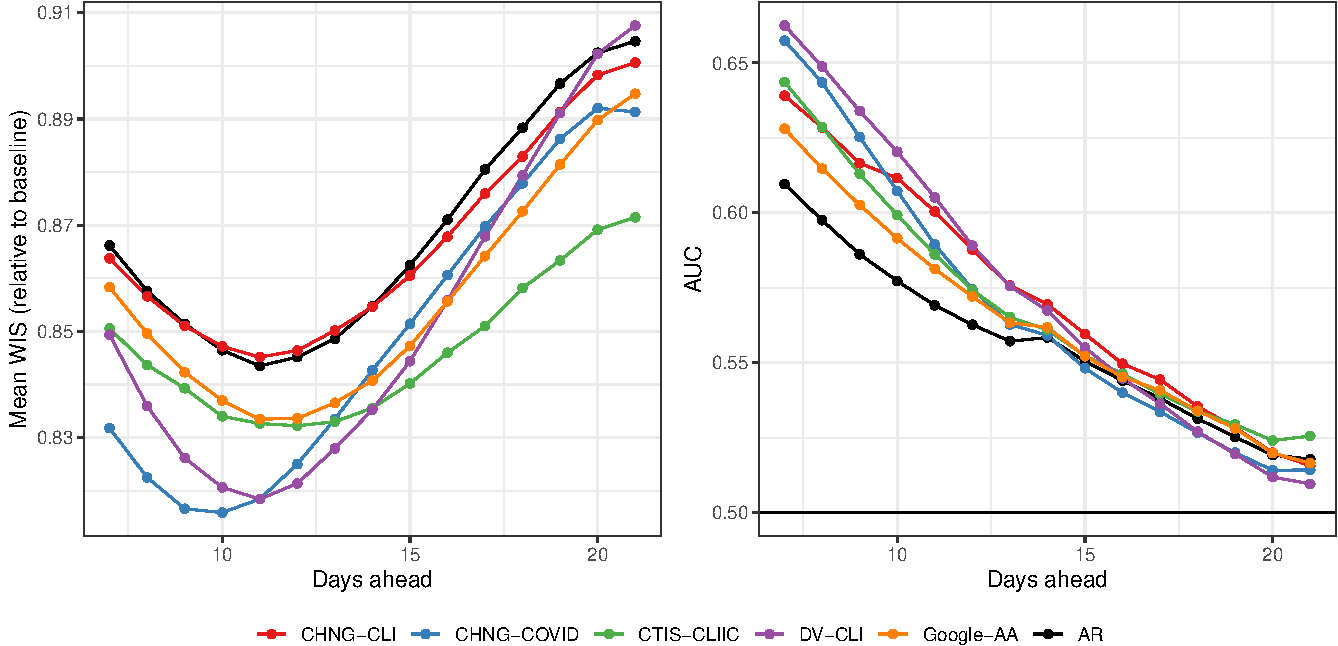
\includegraphics[width=\textwidth]{fig/fcast-hot-combo-1.pdf}
  \caption{Main results for both tasks. Left: average WIS for each forecast
    model, over all forecast dates and all HRRs, divided by the average WIS
    achieved by a baseline model (a probabilistic version of the flat-line
    forecaster).  Right: area under the curve for each hotspot prediction model,
    calculated over all prediction dates and all HRRs.  Here and in all figures
    we abbreviate CTIS-CLI-in-community by CTIS-CLIIC.  
  }  
  \label{fig:forecast}
\end{figure*}

Figure~\ref{fig:forecast} (left panel) displays evaluation results for
forecasting, stratified by ahead value and averaged over all HRRs and forecast
dates.  Shown is the average WIS for each forecast model divided by that from a
baseline model, which is basically a flat-line forecaster (its median forecast
for $Y_{\ell,t+a}$ is always $Y_{\ell,t}$, with predicted quantiles defined
around this based on historical variation). This is the same baseline model as
in the COVID-19 Forecast Hub. Here, we use the baseline model in order to scale
mean WIS so that it gets put on an interpretable, unitless scale.  In the
figure, we can see that all curves are below 1, which means (smaller WIS is
better) that all of the models, including AR, outperform the baseline on average
over the forecasting period.  On the other hand, the models deliver at best an
improvement of about 20\% in average WIS over the baseline model, with this gap
narrowing to about 10\% at the largest ahead values, illustrating the difficulty 
of the forecasting problem.

We can also see from the figure that CHNG-COVID and DV-CLI offer the biggest
gains over AR at small ahead values, followed by CTIS-CLI-in-community and
Google-AA, with the former providing the biggest gains at large ahead values.
The CHNG-CLI model performs basically the same as AR.  This is likely due to the
fact that CHNG-CLI suffers from volatility due to backfill.  The evidence for
this explanation is twofold: (1) the CHNG-CLI model benefits from a more robust
method of aggregating WIS (geometric mean; shown in the supplement); and (2)
when we train and make predictions on finalized data, it handily beats AR, on
par with the best-performing models (also shown in the supplement).  

Figure~\ref{fig:forecast} (right panel) displays the results for hotspot
prediction, again stratified by ahead value and averaged over all HRRs and
prediction dates.  We can see many similarities to the forecasting results (now
larger AUC is better). For example, CHNG-COVID and DV-CLI offer the biggest
improvement over AR, and all models, including AR, degrade in performance
towards the baseline (in this context, a classifier based on random guessing,
which achieves an AUC of 0.5) as the ahead values grow, illustrating the
difficulty of the hotspot prediction problem. A clear difference, however, is
that the CHNG-CLI model performs quite well in hotspot prediction, close to the
best-performing indicator models for many of the ahead values. This may be
because volatility in the CHNG-CLI indicator plays less of a role in the
associated logistic model's predicted probabilities (in general, a sigmoid
function can absorb a lot of the variability in its input).

\subsection{Implicit Regularization Hypothesis}

One might ask if the benefits we observe in forecasting and hotspot
prediction have anything to do with the actual indicator themselves. A plausible  
alternative explanation is that the indicators are simply providing \textit{implicit
  regularization} on top of the basic AR model, in the same way any noise
variable might, when we include them as lagged features in
\eqref{eq:forecast_ar_x} and \eqref{eq:hotspot_ar_x}. 

To test this hypothesis, we reran all of the prediction experiments but with
$X_{\ell,t}$ in the each indicator models replaced with suitable random noise
(bootstrap samples from a signal's history).  The results, shown and explained
more precisely in the supplement, are vastly different (worse) than the original
set of results.  In both forecasting and hotspot prediction, the ``fake''
indicator models offered essentially no improvement over the pure AR model,
which strongly rejects (informally speaking) the implicit regularization
hypothesis.        

On the topic of regularization, it is also worth noting that the use of 
$\ell_1$ regularization (tuned by cross-validation) in fitting any of the models
in \eqref{eq:forecast_ar}, \eqref{eq:forecast_ar_x}, \eqref{eq:hotspot_ar}, or 
\eqref{eq:hotspot_ar_x} did not generally improve their performance
(experiments not shown).  This is likely due to the fact that the number of
training samples is large compared to the number of features (6,426 training
samples and only 3--6 features). 
% DJM: and that proper CV requires longer training windows, exacerbating the
% nonstationarity, a scenario in which its behavior is poorly understood.

\subsection{Evaluation in Up, Down, and Flat Periods}

\begin{figure*}[t]
  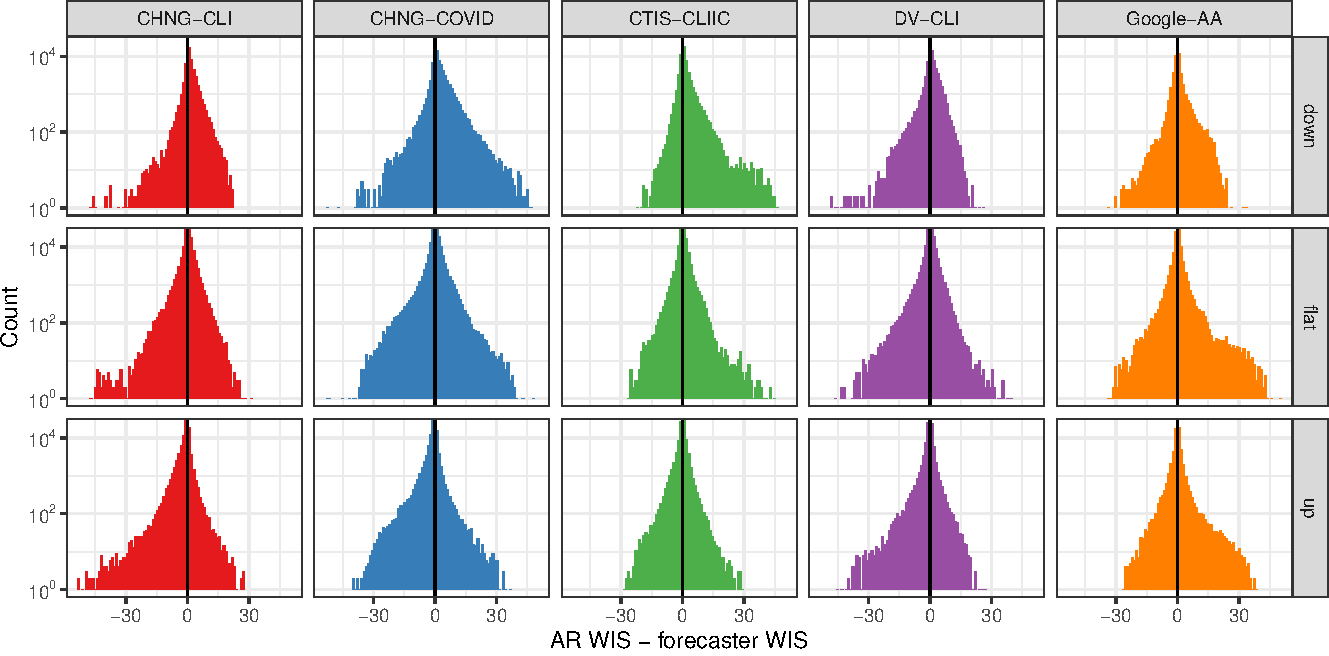
\includegraphics[width=\textwidth]{fig/upswing-histogram-1.pdf}
  \caption{Histogram of the difference in WIS for the AR model and that for each
    indicator model, stratified by up, down, or flat period, measured in terms
    of case trends. Note that \textit{larger} differences here are better for
    each indicator model.  The y-axis is on the log scale to emphasize tail 
    behavior.}   
  \label{fig:up_down_flat}
\end{figure*}

The course of the pandemic has played out quite differently across space and
time. Aggregating case rates nationally shows three pronounced waves, but the
behavior is more nuanced at the HRR level.  Figure \ref{fig:trajectory} is a
single example of a forecast in a period of relatively flat case trends, as New
York City enters what would become its second wave. The AR forecaster's 50\%
prediction interval contains this upswing, but its forecasted median is clearly
below the finalized case data.  Unfortunately, this behavior is fairly typical
of all forecasters: during upswings, the forecasted median tends to fall below 
the target, while the reverse is true during downswings.

Figure~\ref{fig:up_down_flat} shows histograms of the differences in WIS of the 
AR model and each indicator model, where we stratify these differences by
whether the target occurs during a period of increasing cases rates (up),
decreasing case rates (down), or flat case rates (flat). To define the
increasing period, we use the same definition we used for the hotspot task in
Table \ref{tab:analysis_tasks}.  Therefore all hotspots are ``up'', while all
non-hotspots are either ``flat'' or ``down''.  For the ``down'' scenario, we 
simply use the opposite of the hotspot definition: $Y_{\ell,t}$ decreases by
more than 20\% relative to the preceding week.  

While the performance of all forecasters, including AR, will generally degrade
in up periods, different models exhibit different and interesting patterns.
CHNG-CLI, CHNG-COVID, Google-AA, and especially CTIS-CLI-in-community have
large right tails (displaying improvements over AR) during the down periods. 
Google-AA and CTIS-CLI-in-community have large right tails during the flat
periods. CHNG-CLI and DV-CLI have large left tails (poor forecasts relative to
AR) in flat and up periods.  Google-AA is the only model that outperforms
the AR model, on average, over up periods.  Overall, the indicators seem to help
more during flat or down periods than up periods, with the exception of
Google-AA.    

The supplement pursues this analysis further.  For example, we examine
classification accuracy and log-likelihood for the hotspot task and find a
similar phenomenon: the indicators considerably improve accuracy or
log-likelihood during flat or down periods, with more mixed behavior during up
periods when CHNG-CLI, CHNG-COVID, and DV-CLI, in particular, lead to decreased  
performance.

\subsection{Effects of Leading or Lagging Behavior}

\begin{figure}[t]
  \centering
  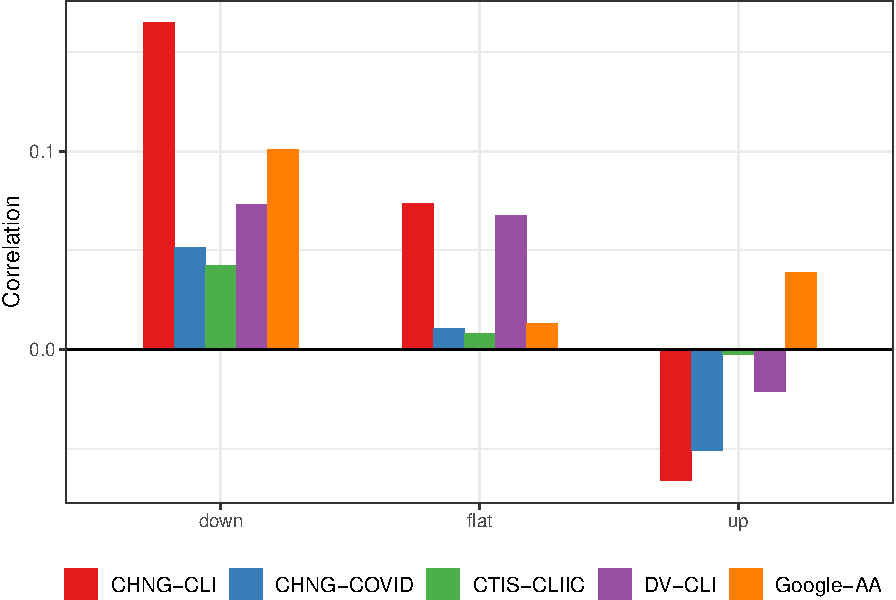
\includegraphics[width=.5\columnwidth]{fig/leading-only-1.pdf}
  \caption{Correlation of the difference in WIS with the ``leadingness'' of the
    indicator at the target date, stratified by up, down, or flat period.} 
  \label{fig:leading}
\end{figure}

As described in the methods section, each of the indicators we examine could be
said to measure aspects of disease progression that would precede a positive
test. That is, we imagine that these signals should ``lead'' cases. It is
entirely reasonable to imagine that, prior to an increase of confirmed COVID-19
tests reported by a public health authority in a particular location, we would
see an increase in medical insurance claims for COVID-related outpatient
visits. However, it may well be the case that such behavior is different
during different periods. In fact, we find empirically that the ``leadingness''
of an indicator (degree to which it leads case activity) tends to be more
pronounced in down or flat periods than in up periods, a plausible explanation 
for the decreased performance in up periods noted above.

In the supplement, we show how to define a quantitative score to measure the
leadingness of an indicator, at any time $t$ and any location $\ell$, based on
cross correlations to case rates over a short time window around $t$.
The higher this score, the greater it ``leads'' case activity.  Figure 
\ref{fig:leading} displays correlations between the leadingness score of an 
indicator and the WIS difference (AR model minus an indicator model), stratified
by whether the target is classified as up, down, or flat.  One would naturally
expect that the WIS difference would be positively correlated with leadingness.
Somewhat surprisingly, this relationship turns out to be strongest in down
periods and weakest in up periods.  In fact, it is very nearly the case that for
each indicator, the strength of correlations only decreases as we move from down
to flat to up  periods.  In the supplement, we extend this analysis by studying 
analogous ``laggingness'' scores, but we do not find as clear patterns. 

\section{Discussion}

Can auxiliary indicators improve COVID-19 forecasting and hotspot prediction
models?  Our answer, based on analyzing five auxiliary indicators from the
COVIDcast API (defined using from medical insurance claims, internet-based
surveys, and internet search trends) is undoubtedly ``yes''. However, there are
levels of nuance to such an answer that must be explained.  None of the
indicators that we have investigated appear to be the ``silver bullet'' that one
might have hoped for, revolutionizing the tractability of the prediction
problem, rendering it easy when it was once hard (in the absence of auxiliary
information).  Rather, the gains in accuracy from the indicator models (over an
autoregressive model based only on past case rates) appear to be nontrivial, and
consistent across modes of analysis, but modest.  In forecasting, the indicator
models are found to be most useful in periods in which case rates are flat or
trending down, rather than periods in which case rates are trending up (as one
might hope to see is the benefit provided by a hypothetical ``leading
indicator'').

As described previously, it is likely that we could improve the indicator models
by using location-specific effects, as well as using nowcasting techniques to
estimate finalized indicator values before we use them as features (to account
for backfill in the claims-based signals in particular).  Beyond this, it is
certainly possible that more sophisticated models for forecasting or hotspot
prediction would lead to different results, and possibly even different
insights. Natural directions to explore include using multiple indicators in a
single model, allowing for interaction terms, and leveraging HRR demographics or
mobility patterns.  That said, we are doubtful that more sophisticated modeling
techniques would change the ``topline'' conclusion---that auxiliary indicators
can provide nontrivial, consistent, but modest gains in forecasting and hotspot
prediction. Whether a more sophisticated model would be able to leverage the
indicators in such a way as to change some of the finer conclusions (e.g., by 
offering clear improvements in periods in which cases are trending up) is less 
clear to us.

We reiterate the importance of using vintage data for rigorous backtesting. Data
sources that are relevant to public health surveillance are often subject to
revision, sometimes regularly (such as medical claims data) and sometimes
unpredictably (such as COVID-19 case reports).  When analyzing models that are
designed to predict future events, if we train these models and make predictions
using finalized data, then we are missing a big part of the story.  Not only
will our sense of accuracy be unrealistic, but certain models may degrade by a
greater or lesser extent when they are forced to work with vintage data, so 
backtesting them with finalized data may lead us to make modeling decisions that
are suboptimal for true test-time performance.    

In this paper, we have chosen to consider only very simple forecasting models,
while devoting most of our effort to accounting for as much of the complexity of
the underlying data and evaluation as possible.  In fact, our paper is as much
about demonstrating how one might address questions about model comparisons and
evaluation in forecasting and hotspot prediction in general, as it is about
providing rigorous answers to such questions in the context of COVID-19 case
rates in particular.  We hope that others will leverage our framework, and build
on it, so that it can be used to guide work that advances the frontier of
predictive modeling for epidemics and pandemics.

\subsubsection*{Acknowledgements}
We thank Matthew Biggerstaff, Logan Brooks, Johannes Bracher, Michael  
Johansson, Evan Ray, Nicholas Reich, and Roni Rosenfeld for several
enlightening conversations about forecasting, scoring, and evaluation.  
This material is based on work supported by gifts from Facebook, Google.org,
the McCune Foundation, and Optum; Centers for Disease Control and Prevention
(CDC) grant U01IP001121; the Canadian Statistical Sciences Institute; National 
Sciences and Engineering Research Council of Canada (NSERC) grant
RGPIN-2021-02618; and National Science Foundation Graduate Research
Fellowship Program (NSF GRFP) award DGE1745016. 

%\showacknow{} % Display the acknowledgments section

% Bibliography
\bibliographystyle{unsrtnat}
\bibliography{../../common/covidcast.bib}

\clearpage

\appendix

\section*{Supplemental information}




\section{Finalized Versus Vintage Data}

The goal of this section is to quantify the effect of not properly accounting
for the question of ``what was known when'' in performing retrospective
evaluations of forecasters.  Figures \ref{fig:fcast-finalized} and
\ref{fig:hot-finalized} show what Figures 3 and 4 in the main paper would have
looked like if we had simply trained all models using the finalized data rather
than using vintage data.  This comparison can be seen more straightforwardly in
Figures \ref{fig:fcast-honest-v-finalized} and \ref{fig:hot-honest-v-finalized},
which show the ratio in performance between the vintage and finalized versions.
When methods are given the finalized version of the data rather than the version
available at the time that the forecast would have been made, all methods appear
(misleadingly) to have better performance than they would have had if run
prospectively.  For example, for forecasting case rates 7-days ahead, the WIS of
all methods is at least 8\% larger than what would have been achieved using
finalized data.  This effect diminishes as the forecasting horizon increases,
reflecting the fact that longer-horizon forecasters rely less heavily on recent
data than very short-horizon forecasters.  Crucially, some methods are
``helped'' more than others by the less scrupulous retrospective evaluation,
underscoring the difficulty of avoiding misleading conclusions when performing
retrospective evaluations of forecasters.

\chngcli~(and, to a lesser extent, the other claims-based signals) is the most
affected by this distinction, reflecting the latency in claims-based reporting.
This underscores the importance of efforts to provide ``nowcasts'' for claims
signals (which corresponds to a 0-ahead forecast of what the claims signal's
value will be once all data has been collected). Looking at the \chngcli~and
\dv~curves in Figure \ref{fig:fcast-finalized}, we can see that they perform
very similarly when trained on the finalized data.  This is reassuring because
they are, in principle, measuring the same thing (namely, the percentage of
outpatient visits that are primarily about COVID-related symptoms), but based on
data from different providers.  The substantial difference in their curves in
Figure 3 of the main paper must therefore reflect their having very different
backfill profiles. 
  
While using finalized rather than vintage data affects \dv~the least for
forecasting, it is one of the most affected methods for the hotspot problem.
This is a reminder that the forecasting and hotspot problems are fundamentally
different problems.  For example, the hotspot problem does not measure the
ability to distinguish between flat and downward trends.

Even the \ar~model is affected by this distinction, reflecting the fact that the
case rates themselves (i.e., the response values) are also subject to revision.
The forecasters based on indicators are thus affected both by revisions to the
indicators and by revisions to the case rates.  And in the case of the
\gs~model, in which we only used finalized values for the \gs~indicator, the
difference in performance can be wholly attributed to revisions of case rates. 

\section{Robust Aggregation}

In this section, we consider using the geometric mean instead of the usual
(arithmetic) mean when aggregating the weighted interval score (WIS) across
location-time pairs.  Aside from the geometric mean being generally more robust
to large values, there are two reasons why using it may be desirable.  

\begin{enumerate}
\item WIS is right-skewed, being bounded below by zero and having occasional 
  very large values.  Figure \ref{fig:wis-densities} illustrates that the
  densities appear roughly log-Gaussian.  The geometric mean is a natural choice   
  in such a context since it can be viewed as a measure of centrality on the log
  scale (it is the exponential of the arithmetic mean of log values).
\item In the main paper, we report the ratio of the mean WIS of a forecaster to
  the mean WIS of the baseline forecaster. Another choice could be to take the
  mean of the ratio of WIS values for the two methods. This latter choice would
  penalize a method less for doing poorly where the baseline forecaster also
  does poorly.\footnote{In a sense, this is implicitly estimating a
    nonparametric space-time effect for forecaster error, and assuming that has
    a shared, multiplicative contribution to forecaster errors.  That is, if one
    imagines that a forecaster's WIS is composed of multiplicative space-time
    effects $S_{\ell,t}$ shared across all forecasters,
    \smash{$\WIS(F_{\ell,t,f},Y_{\ell,t}) = S_{\ell,t} E_{f,t}$} with
    \smash{$E_{f,t}$} a forecaster-specific error, then taking the ratio of
    individual WIS values cancels these space-time effects.}  Using instead the
  geometric mean makes the order of aggregation and scaling immaterial since the
  ratio of geometric means is the same as the geometric mean of ratios.
\end{enumerate}

Figure \ref{fig:fcast-adjusted} uses the geometric mean for aggregation.
Comparing this with Figure 3 in the main paper, we see that the main conclusions
are largely unchanged; however, \chngcli~now appears better than \ar.  This
behavior would be expected if \chngcli's poor performance is attributable to a
relatively small number of large errors (as opposed to a large number of
moderate errors).  Indeed, Figure 5 of the main paper further corroborates this,
in which we see the heaviest left tails occur for \chngcli.

\section{Comparing COVID-19 Forecast Hub Models}

Since July of 2020, modelers have been submitting real-time forecasts of
COVID-19 case incidence to the COVID-19 Forecast Hub \cite{ForecastHub}. This 
(along with forecasts of hospitalizations and deaths collected in the same Hub)
serves as the source of the CDC's official communications on COVID forecasting. 

Our goal in this section is to compare the AR model and indicator models to
those in the Hub, in terms of forecast errors aggregated over the same forecast
tasks, to give a clear sense for how robust and effective the models we choose
to investigate in the paper are relative to those in common operational use.
This was prompted by a question from an anonymous reviewer of this paper, who
asked why we chose to build our analysis of indicator utility around the AR
model in the first place, and why we did not build it around others (say, the
SIR model or more complex mechanistic models of disease transmission) that have 
occupied more of the spotlight over the course of the pandemic.  The analysis
presented here corroborates the claim that, while simple, the AR model, properly
trained---using a quantile loss to directly estimate multiple conditional
quantiles, a trailing training window of 21 days, pooling across all locations
jointly, and fitting to case rates rather than counts (as we do in all our
models in the main paper)---can be robust and effective, performing
competitively many of the top models from COVID-19 Forecast Hub, including the
Hub ensemble model.

The closest forecast target in the Hub to that used in the main paper is 
state-level case incidence over an epiweek---defined by the sum of new case
counts reported between a Sunday and the following Saturday (inclusive). Our
forecast target, recall, is a 7-day trailing average of COVID-19 case incidence
rates at the HRR level, which is different in three regards:

\begin{enumerate}
\item temporal resolution (daily versus weekly);
\item geographic resolution (HRRs versus states); 
\item scale (rates versus counts).
\end{enumerate}

While the first and third of these differences could be easily addressed post 
hoc---meaning, we can take always take our model's output and multiply it by 
7 in order to track the incidence over any given trailing week, and rescale it
per location by population to bring it to the count scale---the second
difference is not easy to adjust post hoc due to nonlinearity of the quantiles
(a quantile of a linear combination of random variables is not simply the linear
combination of their quantiles, but rather, depends intricately on the
correlations between the random variables).    

Therefore, to make a comparison to models in the Hub as direct as possible, we
retrained our models over the same forecast period as in the main paper, and
with the same general setup entirely, except at the state rather than HRR level.
We then rescaled them post hoc to account for the different temporal resolution
and the rate versus count scale (first and third points in the above list).  The
results are given in Figure \ref{fig:compare-to-hub}.  The evaluation was
carried out exactly as in the main paper, and the figure displays both mean WIS
and geometric mean WIS, as a function of ahead, relative to the baseline model.
Furthermore, to account for missingness (not all teams submitted forecasts to
the Hub for all locations and ahead values for the entire period), we first
dropped any forecaster than submitted for less than 6 weeks, and then restricted
the aggregation metrics (mean or geometric mean) to errors from commonly
available forecast tasks.

By either metric, mean or geometric mean WIS relative to baseline, we can see  
in Figure \ref{fig:compare-to-hub} that the AR model examined in this paper is 
competitive with top models in the Hub, even outperforming the Hub ensemble
model for smaller ahead values.  The same general conclusion can be drawn for
the indicators models as well.  However, interestingly, a close inspection
reveals that the AR model here is for the most part in the ``middle of the
pack'' when compared to the indicator models, and only the Google-AA model
offers clear improvement over AR for all aheads.  This is likely due to the fact
that at the state level, the signal-to-noise ratio (SNR) is generally higher,
and AR model provides a higher standard (on which to expect improvement using an 
auxiliary indicator), since it is able to extract a clearer signal from past
lags of case rates.  At the HRR level, with lower SNR, using indicators as
simple additional linear features in the AR model probably leads to a variance
reduction that is enough to boost accuracy, but at the state level, perhaps more
sophisticated modeling techniques are needed to extract comparable value from
some of the indicators.

\section{Statistical Significance}

In the introduction of the main manuscript, we gave some reasons that we avoid
making formal statements about statistical significance, preferring instead to
examine the stability of our results in different contexts.  There are strong
reasons to avoid model-based significance tests because the necessary
assumptions about stationarity, independence, and the model being true (or at
least approximately true) are certainly violated.  With those caveats in mind,
we undertake two relatively assumption-lean investigations in this section.  The
first is a sign test for whether the difference between the AR model’s relative
WIS and each other model’s relative WIS is centered at zero.  (Relative WIS here
means scaled by the WIS of the baseline model.)  To mitigate the dependence 
across time (which intuitively seems to matter more than that across space), we
computed these tests in a stratified way, where for each forecast date we run a
sign test on the scaled errors between two models over all 306 HRRs.  The
results are plotted as histograms in Figure \ref{fig:sign-test}.  For this
figure, we use the total relative WIS over all aheads, but the histograms are
largely similar for individual target horizons. If there were no difference, we
would expect to see a uniform distribution. However, for each indicator model, 
we see many more small p-values than would be expected if the null hypothesis
(that the AR model is better) were true. 

Another relatively assumption-lean method of testing for differences in forecast
accuracy is the Diebold-Mariano (DM) test \cite{Diebold:2002, Diebold:2015,
Harvey:1997}. Essentially, the differences between forecast errors are assumed
to have a constant mean and a covariance that depends on time.  Under these
conditions, the asymptotic distribution for the standardized mean of the
differences is limiting normal provided that a heteroskedasticity and
autocorrelation robust estimate of the variance is used.  Using the error as WIS
across all HRRs and horizons (7 to 21 days ahead), we perform the DM test using
both the mean relative to the baseline (as reported in the manuscript) and the
geometric mean relative to the baseline as described above.  The first two rows
of Table \ref{tab:dm-test} displays p-values for the test that each indicator
model is no better than the AR model.  In only a few instances---geometric mean
and mean for the CHNG-CLI model, and mean for the CHNG-COVID model---do the
p-values exceed conventional statistical significance thresholds. 

\section{Bootstrap Results}

As explained in Section 2.B of the main paper, a (somewhat cynical) hypothesis
for why we see benefits in forecasting and hotspot prediction is that the
indicators are not actually providing useful information but they are instead
acting as a sort of ``implicit regularization,'' leading to shrinkage on the
autoregressive coefficients and therefore to less volatile predictions.  To
investigate this hypothesis, we consider fitting ``noise features'' that in
truth have zero relationship to the response.  Recall (from the main paper) that
at each forecast date, we train a model on 6,426 location-time pairs.  Each
indicator model uses 6 features, corresponding to the 3 autoregressive terms and
the 3 lagged indicator values.  To form noise indicator features, we replace
their values with those from a randomly chosen time-space pair (while keeping
the autoregressive features fixed).  In particular, at each location $\ell$ and
time $t$, for the forecasting task we replace the triplet \smash{$(X_{\ell,t},
X_{\ell,t-7}, X_{\ell,t-14})$} in Eq.\ (3) of the main
paper with the triplet \smash{$(X_{\ell^*,t^*}, X_{\ell^*,t^*-7},
  X_{\ell^*,t^*-14})$}, where $(\ell^*,t^*)$ is a location-time pair sampled with
replacement from the 6,426 total location-time pairs.  Likewise in the hotspot 
prediction task, we replace the triplet \smash{$(X_{\ell,t}^\Delta,
  X_{\ell,t-7}^\Delta, X_{\ell,t-14}^\Delta)$} in Eq.\ (5) of the main paper with
\smash{$(X_{\ell^*,t^*}^\Delta, X_{\ell^*,t^*-7}^\Delta,
  X_{\ell^*,t^*-14}^\Delta)$}.  Figures
\ref{fig:fcast-booted}--\ref{fig:hot-booted} show the results.  No method
exhibits a noticeable performance gain over the \ar~method, leading us to
dismiss the implicit regularization hypothesis. 

\section{Upswings and Downswings}

In this section, we provide extra details about the up/down/flat analysis
described in the main manuscript. Figure \ref{fig:upswing-summary} shows the
overall results, examining the average difference $\WIS(AR) - \WIS(F)$ in
period. Figure \ref{fig:hotspots-upswing-downswing} shows the same information
for the hotspot task. On average, during downswings and flat periods, the
indicator models have lower classification error and higher log likelihood than
the AR model. For hotspots, both Google-AA and CTIS-CLIIC perform better than
the AR model during upswings, in contrast to the forecasting task, where only
Google-AA improves. For a related analysis, Figure \ref{fig:cor-wis-ratio} shows
histograms of the Spearman correlation (Spearman's $\rho$, a rank-based measure
of association) between the $\WIS(F)/\WIS(AR)$ and the magnitude of the
swing. Again we see that case rate increases are positively related to
diminished performance of the indicator models.

One hypothesis for diminished relative performance during upswings is that the
AR model tends to overpredict downswings and underpredict upswings. Adding
indicators appears to help avoid this behavior on the downswing but not as much
on upswings. Figure \ref{fig:upswing-corr-table} shows the correlation between
between $\WIS(AR) - \WIS(F)$ and the difference of their median forecasts.
During downswings, this correlation is large, implying that improved relative
performance of $F$ is related to making lower forecasts than the AR model. The
opposite is true during upswings. This is largely to be expected. However, the
relationship attenuates in flat periods and during upswings. That is, when
performance is better in those cases, it may be due to other factors than simply
making predictions in the correct direction, for example, narrower confidence
intervals.

It is important to note, that even though some indicators, notably CHNG-COVID 
and CHNG-CLI underperform relative to the AR model during upswings, all models 
dramatically outperform the baseline in such periods. Figure 
\ref{fig:upswing-summary-remake} shows the performance of all forecasters relative
to the null model. All forecasters suffer relative to the baseline during down 
periods, but the AR is the worst. In contrast, all models beat the baseline
during up periods, even CHNG-COVID and CHNG-CLI, though not by quite as much as the
AR does.

\section{Leadingness and Laggingness}

In Section 2.D of the main text, we discuss the extent to which the indicators
are leading or lagging case rates during different periods. To define the amount
of leadingness or laggingness at location $\ell$, we use the cross correlation
function (CCF) between the two time series. The $\CCF_\ell(a)$ of an indicator
$X_{\ell}$ and case rates $Y_{\ell}$ is defined as
% \[
% \CCF_{\ell,t}(a) = \frac{1}{n_a} \sum_{i=1}^{n_a} \left( ( X_{\ell,t,i+a} -
%   \overline{X}_{\ell,t}) / s^{X}_{\ell,t}\right) \left( ( Y_{\ell,t,i} -
%   \overline{Y}_{\ell,t}) / s^{Y}_{\ell,t}\right), 
% \]
% where $n_a$ is the number of available time points when $X_{\ell,t}$ has been
% shifted in time by $a$ days, and $\overline{X}_{\ell,t}$, $s^X_{\ell,t}$
% are the sample mean and
% standard deviation of $X_{\ell,t}$ (respectively $Y_{\ell,t}$). The result is a
their Pearson correlation where $X_\ell$ has been aligned with the values of
$Y_{\ell}$ that occurred $a$ days earlier.  Thus, for any $a>0$,
$\CCF_{\ell}(a)>0$ indicates that $Y_{\ell,t}$ is moving together with
$X_{\ell,t+a}$.  In this case we say that $X_{\ell}$ is lagging $Y_{\ell}$. For
$a<0$, $\CCF_{\ell}(a)>0$ means that $Y_{\ell,t}$ is positively correlated with
$X_{\ell,t-a}$, so we say that $X_{\ell}$ leads $Y_{\ell}$.

Figure \ref{fig:ccf-dv-finalized} shows the standardized signals for the HRR
containing Charlotte, North Carolina, from August 1, 2020 until the end of
September. These are the same signals shown in Figure 1 in the manuscript but
using finalized data. To define ``leadingness'' we compute $\CCF_{\ell}(a)$ (as
implemented with the R function {\tt ccf()}) for each $a\in \{-15,\ldots,15\}$
using the 56 days leading up to the target date. This is the same amount of data
used to train the forecasters: 21 days of training data, 21 days to get the
response at $a=21$, and 14 days for the longest lagged value. The orange dashed
horizontal line represents the 95\% significance threshold for correlations
based on 56 observations. Any correlations larger in magnitude than this value
are considered statistically significant under the null hypothesis of no
relationship. We define leadingness to be the sum of the significant
correlations that are leading (those above the dashed line with $a<0$) while
laggingness is the same but for $a>0$. In the figure, there are three
significant correlations on the ``leading'' side (at $a = -5, -4, -3$), so
leadingness will be the sum of those values while laggingness is 0: on September
28 in Charlotte, \dv~is leading cases leading but not lagging.

Figure \ref{fig:lagging-only} shows the correlation between laggingness and the
difference in indicator WIS and AR WIS. Unlike leadingness (Figure 5 in the
manuscript) there is no obvious relationship that holds consistently across
indicators. This is heartening as laggingness should not aid forecasting
performance. On the other hand, if an indicator is more lagging than it is
leading, this may suggest diminished performance.
Figure~\ref{fig:diff-in-lead-lag} shows the correlation of the difference in
leadingness and laggingness with the difference in WIS. The pattern here is
largely similar to the pattern in leadingness described in the manuscript: the
relationship is strongest in down periods and weakest in up periods with the
strength diminishing as we move from down to flat to up for all indicators.

In calculating the CCF and the associated leadingness and laggingness scores, we
have used the finalized data, and we look at the behavior at the target date of
the forecast. That is we are using the same data to evaluate predictive accuracy
as to determine leadingness and laggingness. It should be noted that the
leadingness of the indicator at the time the model is trained may also be
important. Thus, we could calculate separate leadingness and laggingness scores
for the trained model and for the evaluation data and examine their combination
in some way. We do not pursue this combination further and leave this
investigation for future work.

% \section{Examining data in 2021}

% In this section, we investigate the sensitivity of the results to the
% period over which we train and evaluate the models.  In the main
% paper, we end all evaluation on December 31, 2020.  Figures
% \ref{fig:fcast-alldates}--\ref{fig:hot-alldates} show how the
% results would differ if we extended this analysis through March
%   31, 2021. Comparing Figure \ref{fig:fcast-alldates} to Figure 3 of
% the main paper, one sees that as ahead increases most methods now improve
% relative to the baseline forecaster. When compared to other methods, 
% \chngcli~appears much better than
% it had previously; however, all forecasters other than \chngcov~and
% \dv~are performing less well relative to the baseline than before.
% These changes are likely due to the differing nature of the pandemic
% in 2021, with flat and downward trends much more common than upward
% trajectories.  Indeed, the nature of the hotspot prediction problem is
% quite different in this period.  With a 21-day training window, it is
% common for there to be many fewer hotspots in training.

\section{Aggregation Over Time and Space}

Following the suggestion of an anonymous reviewer, we investigate two
other disaggregated versions of the main forecasting result shown in Figure 3 on the
manuscript. The first (Figure \ref{fig:cumulative-mean}) displays the cumulative
error (summed over all horizons) of each forecaster divided by the cumulative
error of the baseline.  This perspective should illustrate how the models
perform over time, drawing attention to any nonstationary behavior.  During the
initial increase in cases in July 2020, CTIS-CLIIC and Google-AA gain a lot
relative to the AR model. All the indicators do much better than the AR model
during the following downturn (the ebb of the second wave). The AR model
actually improves over the indicators in October 2020, before losing a bit in
late November. The second (Figure \ref{fig:cumulative-geo-mean}) repeats this 
analysis but aggregating by Geometric mean as described above and displays a
similar pattern.

Figure \ref{fig:errs-in-space} examines the spatial behavior over the entire
period of the indicator models relative to the AR. For ease of
comparison, we show the percent improvement in each HRR. Negative numbers (blue)
mean that the indicator helped while positives (red) mean that the indicator
hurt forecasting performance. The clear pattern is that in most HRRs, the
indicators improved performance, though usually by small amounts (2.5\%--10\%).
In some isolated HRRs, performance was markedly worse, though there does not
appear to be any particular pattern to these locations.


\begin{figure}

{\centering 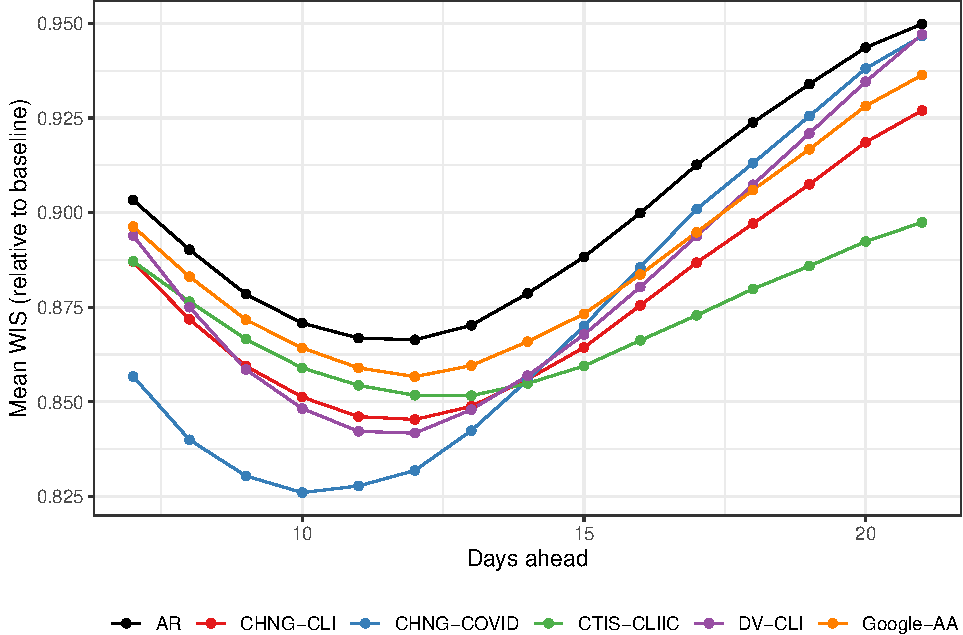
\includegraphics[width=\textwidth]{fig/fcast-finalized-1} 

}

\caption{Forecasting performance using finalized data. Compare to Figure 3 in the manuscript.}\label{fig:fcast-finalized}
\end{figure}

\clearpage

\begin{figure}

{\centering 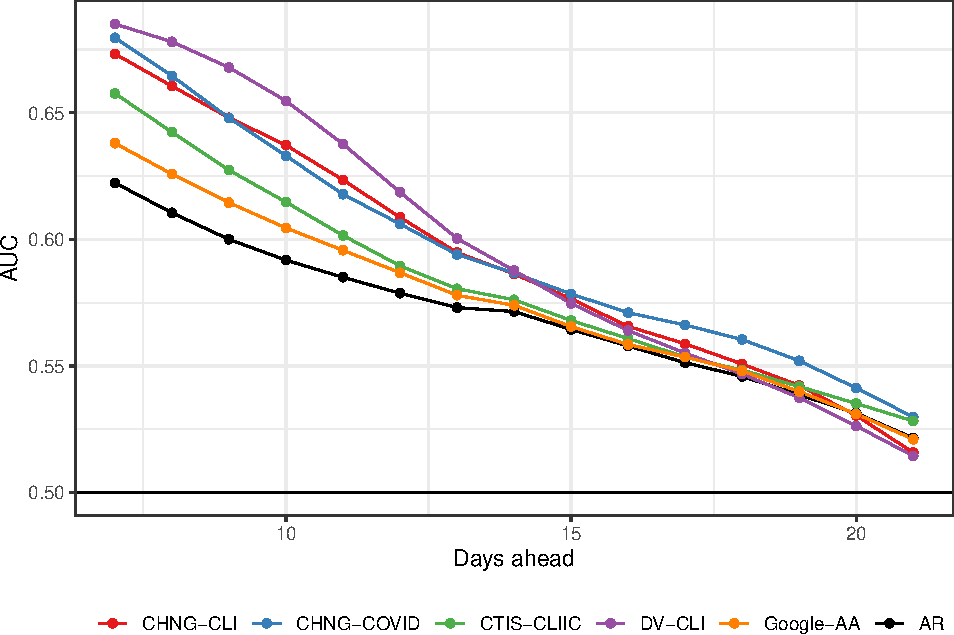
\includegraphics[width=\textwidth]{fig/hot-finalized-1} 

}

\caption{Hotspot prediction performance using finalized data. Compare to Figure 4 in the manuscript.}\label{fig:hot-finalized}
\end{figure}

\clearpage

\begin{figure}

{\centering 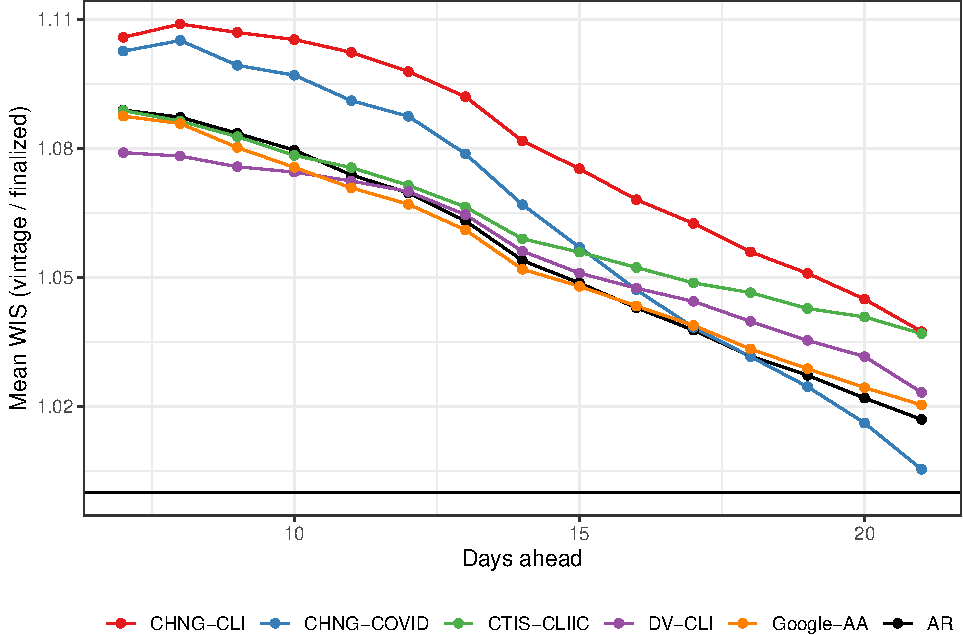
\includegraphics[width=\textwidth]{fig/fcast-honest-v-finalized-1} 

}

\caption{Relative forecast WIS with vintage compared to finalized data. Using finalized data leads to overly optimistic performance.}\label{fig:fcast-honest-v-finalized}
\end{figure}

\clearpage

\begin{figure}

{\centering 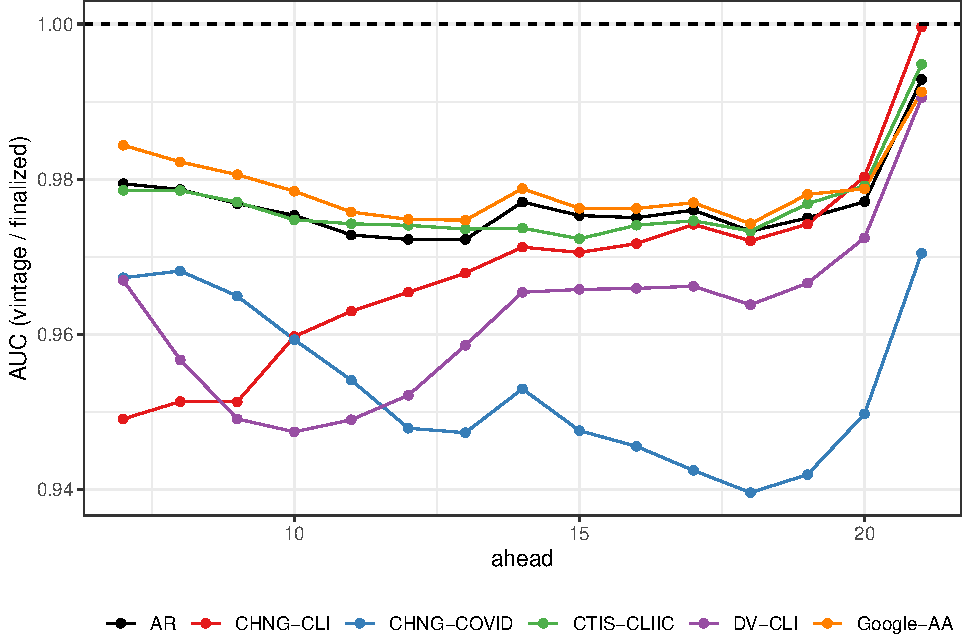
\includegraphics[width=\textwidth]{fig/hot-honest-v-finalized-1} 

}

\caption{Relative AUC with vintage compared to finalized data. Using finalized data leads to overly optimistic hotspot performance.}\label{fig:hot-honest-v-finalized}
\end{figure}

\clearpage

\begin{figure}

{\centering 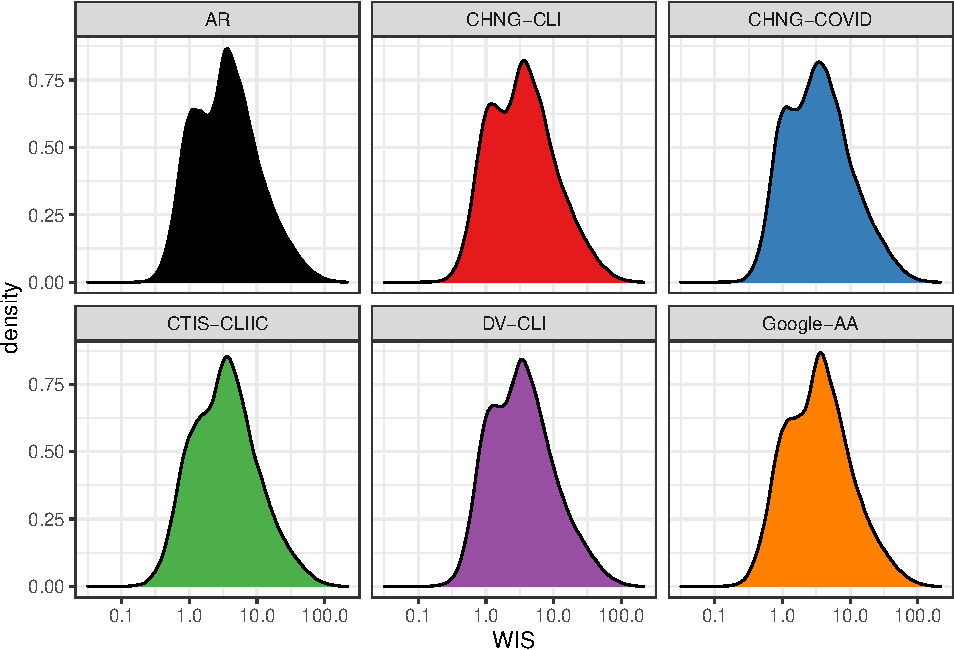
\includegraphics[width=\textwidth]{fig/wis-densities-1} 

}

\caption{Weighted interval score appears to more closely resemble a log-Gaussian distribution.}\label{fig:wis-densities}
\end{figure}

\clearpage

\begin{figure}

{\centering 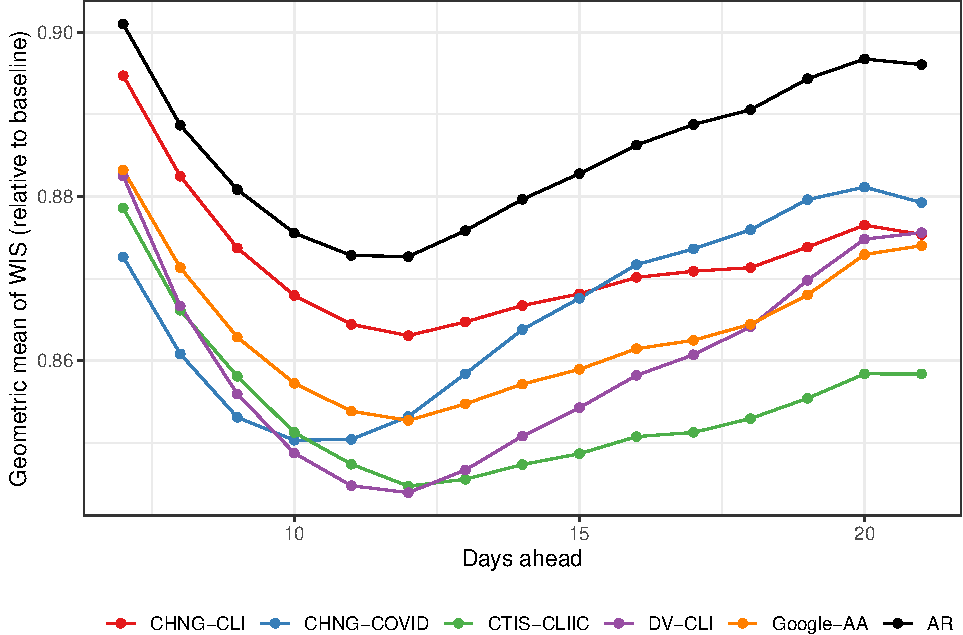
\includegraphics[width=\textwidth]{fig/fcast-adjusted-1} 

}

\caption{Relative forecast performance using vintage data and summarizing with the more robust geometric mean.}\label{fig:fcast-adjusted}
\end{figure}

\clearpage

\begin{figure}

{\centering 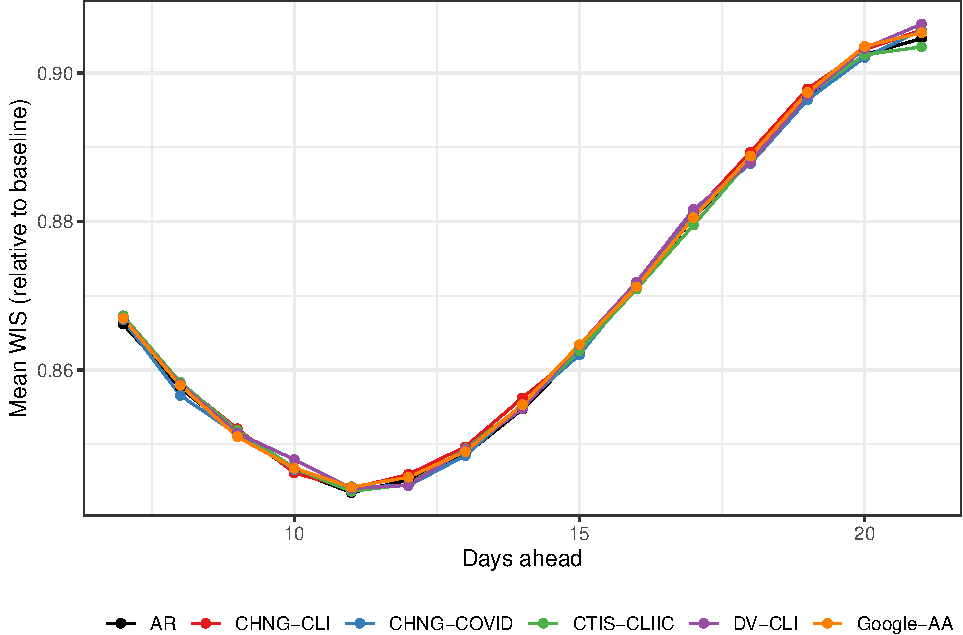
\includegraphics[width=\textwidth]{fig/fcast-booted-1} 

}

\caption{Forecast performance when indicators are replaced with samples from their empirical distribution. Performance is largely similar to the AR model.}\label{fig:fcast-booted}
\end{figure}

\clearpage

\begin{figure}

{\centering 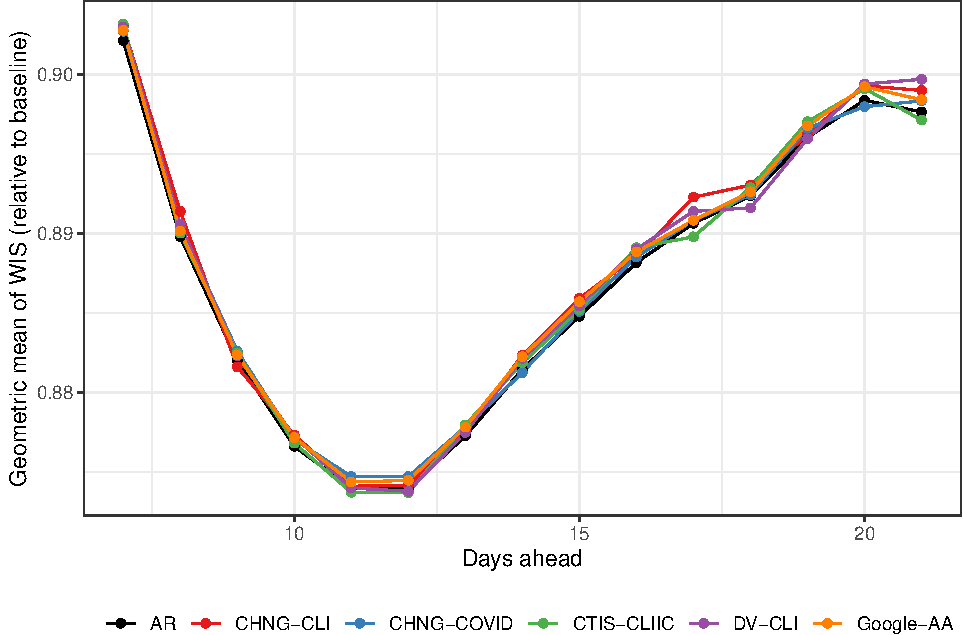
\includegraphics[width=\textwidth]{fig/fcast-booted-adjusted-1} 

}

\caption{Forecast performance as measured with the geometric mean when indicators are replaced with samples from their empirical distribution. Performance is largely similar to the AR model.}\label{fig:fcast-booted-adjusted}
\end{figure}

\clearpage

\begin{figure}

{\centering 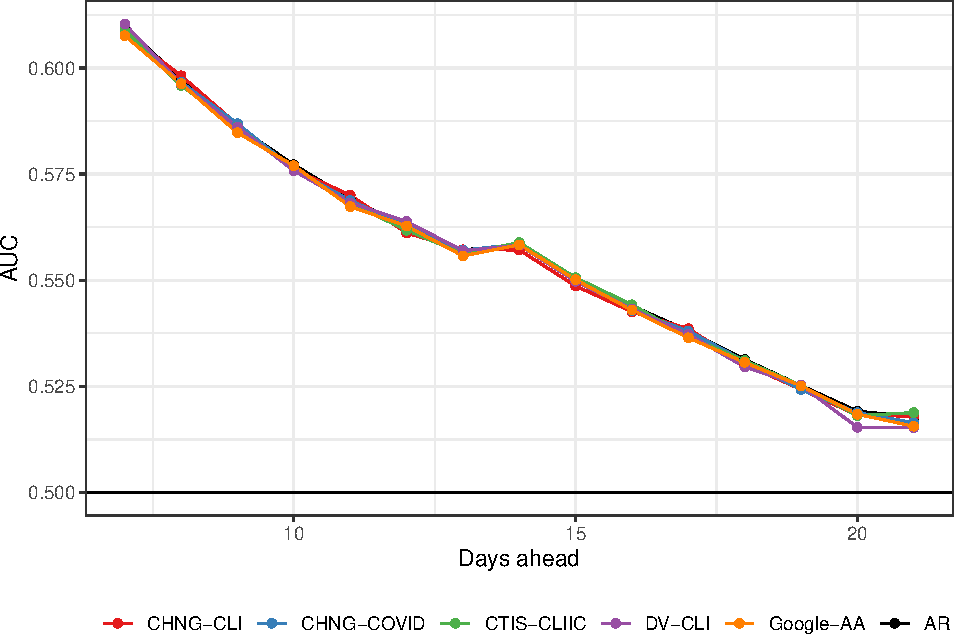
\includegraphics[width=\textwidth]{fig/hot-booted-1} 

}

\caption{Hotspot prediction performance when indicators are replaced with samples from their empirical distribution. Performance is largely similar to the AR model.}\label{fig:hot-booted}
\end{figure}

\clearpage

\begin{figure}

{\centering 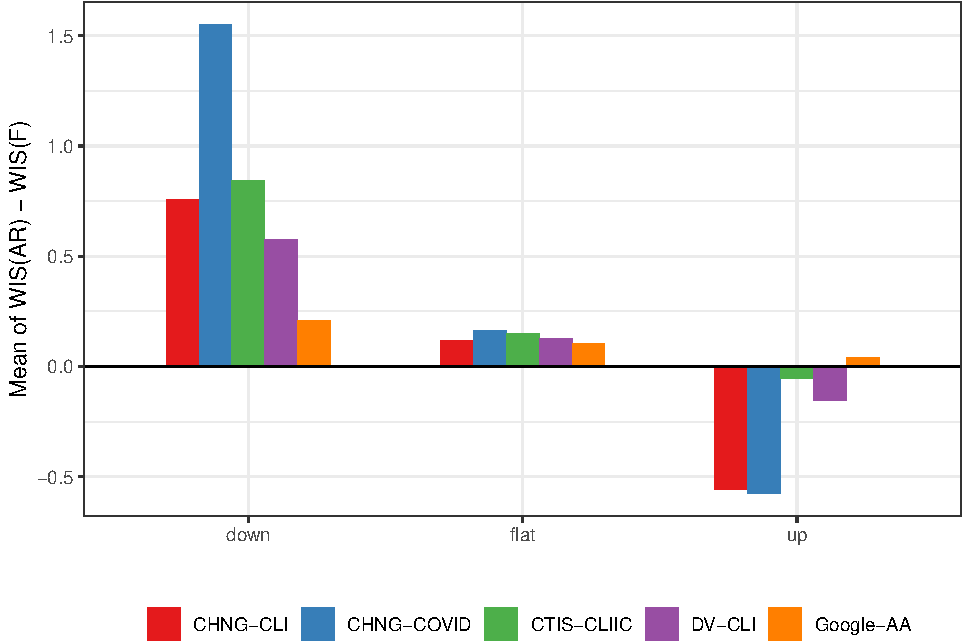
\includegraphics[width=\textwidth]{fig/upswing-summary-1} 

}

\caption{Average difference between the WIS of the AR model and the WIS of the other forecasters. The indicator-assisted forecasters do best during down and flat periods.}\label{fig:upswing-summary}
\end{figure}

\clearpage

\begin{figure}

{\centering 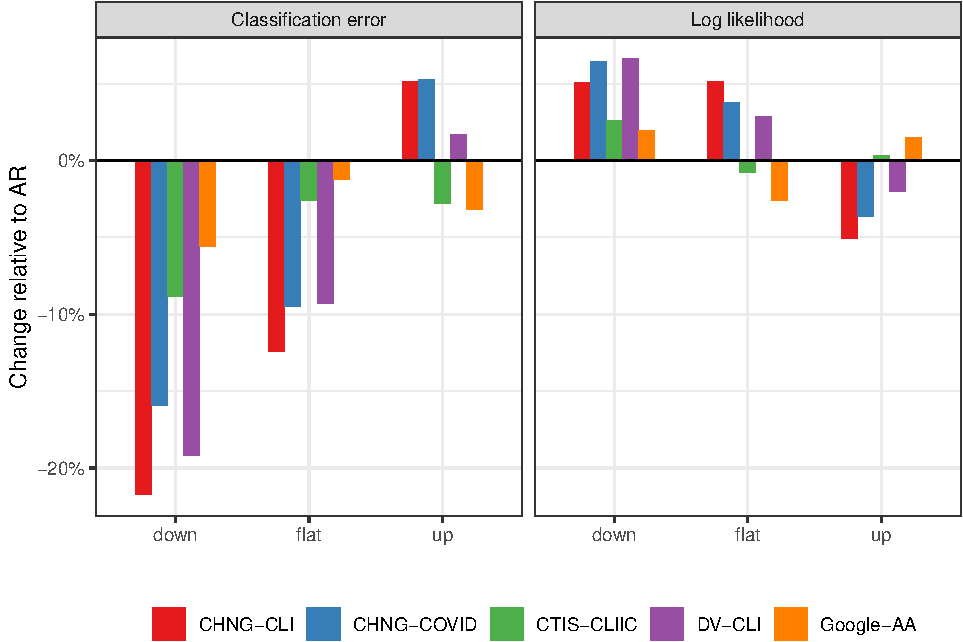
\includegraphics[width=\textwidth]{fig/hotspots-upswing-downswing-1} 

}

\caption{Classification and loglikelihood separated into periods of upswing, downswing, and flat cases. Like the analysis of the forecasting task in the main paper (see Figure 7), performance is better during down and flat periods.}\label{fig:hotspots-upswing-downswing}
\end{figure}

\clearpage

\begin{figure}

{\centering 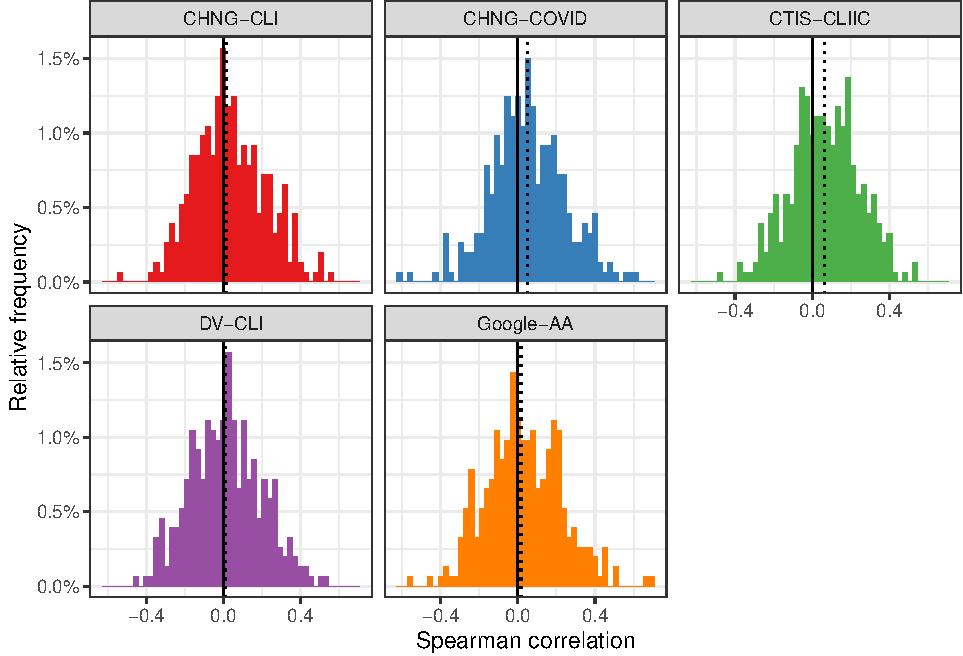
\includegraphics[width=\textwidth]{fig/cor-wis-ratio-1} 

}

\caption{Histograms of the Spearman correlation between the ratio of AR to AR WIS with the percent change in smoothed case rates relative to 7 days earlier.}\label{fig:cor-wis-ratio}
\end{figure}

\clearpage

\clearpage

\begin{figure}

{\centering 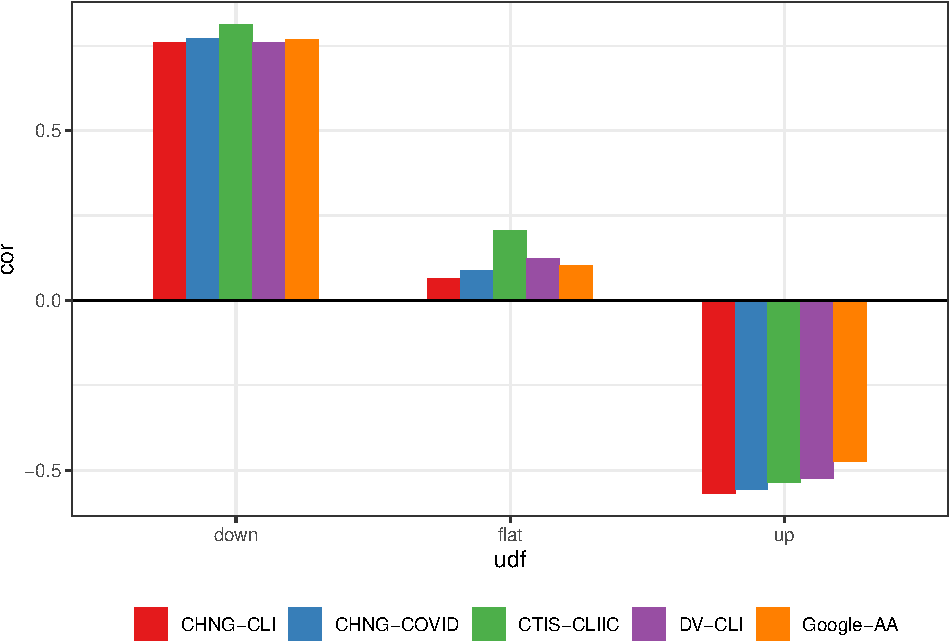
\includegraphics[width=\textwidth]{fig/upswing-corr-table-1} 

}

\caption{Correlation of the difference in WIS with the difference in median predictions for the AR model relative to the indicator-assisted forecaster. In down periods, improvements in forecast risk are highlycorrelated with lower median predictions. The opposite is true in up periods. This suggests, as one might expect that improved performance of the indicator-assisted model is attributable to being closer to the truth then the AR model. This conclusion is stronger in down periods then in up periods.}\label{fig:upswing-corr-table}
\end{figure}

\clearpage

\begin{figure}

{\centering 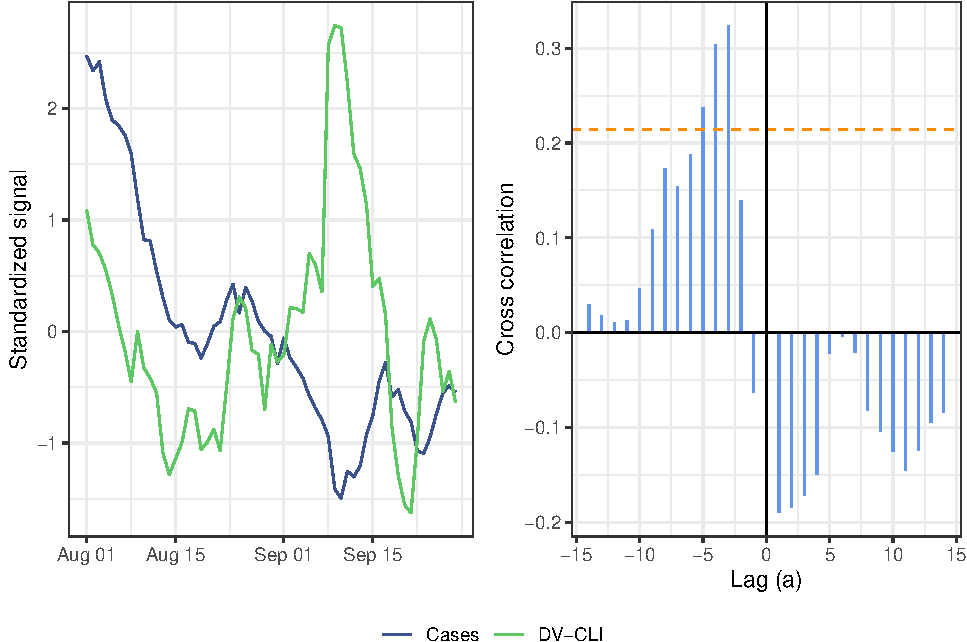
\includegraphics[width=\textwidth]{fig/ccf-dv-finalized-1} 

}

\caption{Illustration of the cross-correlation function between DV-CLI and cases. The left panel shows the standardized signals over the period from August 1 to September 28 (as of May 15, 2021). The right panel shows $\CCF_{\ell}(a)$ for different values of $a$ as vertical blue bars. The orange dashed lines indicate the 95\% significance threshold. By our leadingness/laggingness metric, DV-CLI is leading (but notlagging) cases over this period.}\label{fig:ccf-dv-finalized}
\end{figure}

\clearpage

\begin{figure}

{\centering 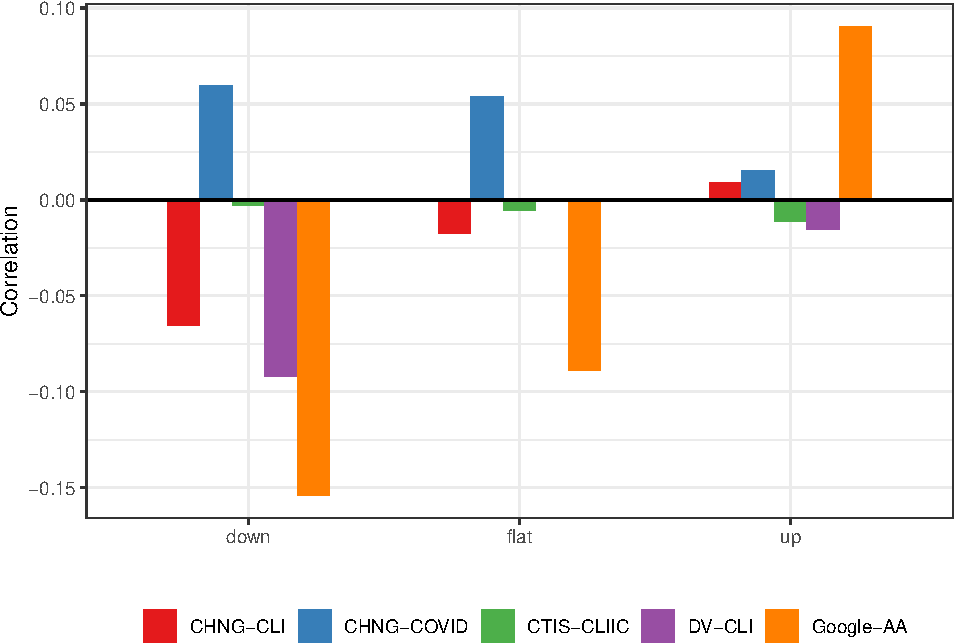
\includegraphics[width=\textwidth]{fig/lagging-only-1} 

}

\caption{Correlation of the difference in WIS with the  laggingness of the indicator at the target date, stratified by up, down, or flat period. Compare to Figure 5 in the manuscript.}\label{fig:lagging-only}
\end{figure}

\clearpage

\begin{figure}

{\centering 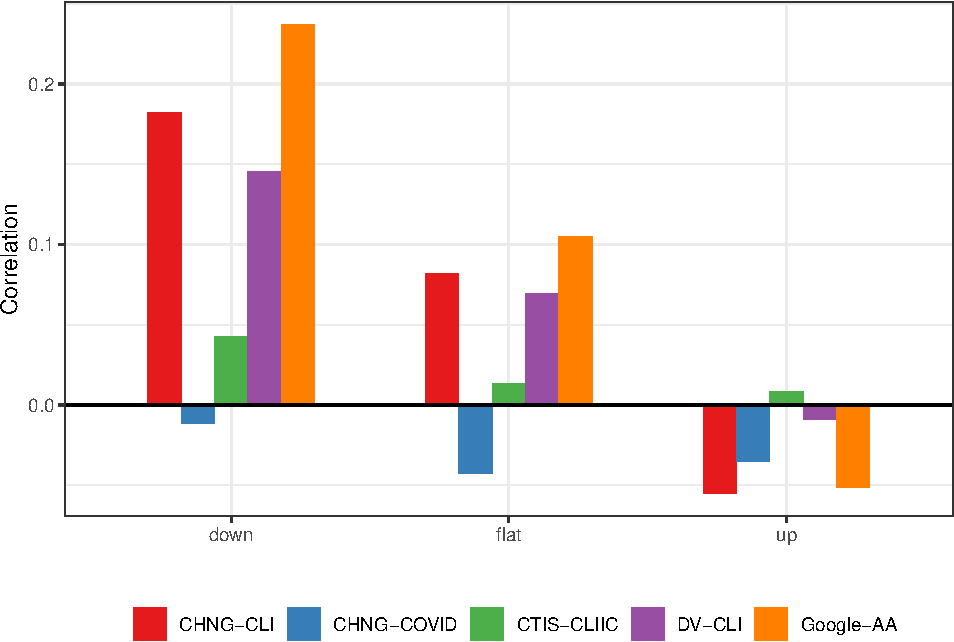
\includegraphics[width=\textwidth]{fig/diff-in-lead-lag-1} 

}

\caption{Correlation of the difference between leadingness and laggingness with the difference in WIS. The relationship is essentially the same as described in the manuscript and shown in Figure 5.}\label{fig:diff-in-lead-lag}
\end{figure}

\clearpage

\begin{figure}

{\centering 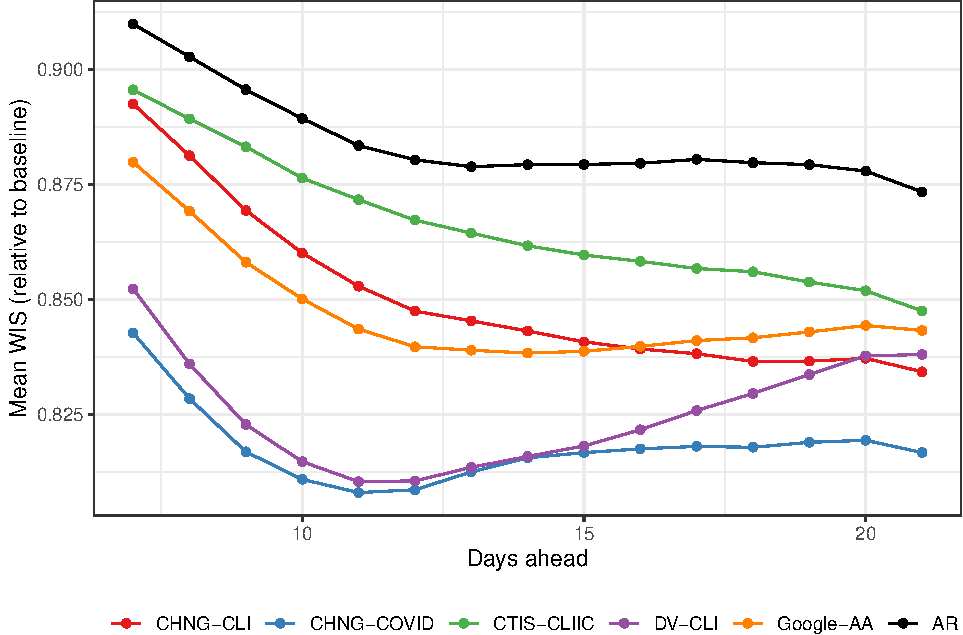
\includegraphics[width=\textwidth]{fig/fcast-alldates-1} 

}

\caption{Forecast performance over all periods. Performance largely improves for all forecasters with the inclusion of data in 2021.}\label{fig:fcast-alldates}
\end{figure}

\clearpage

\begin{figure}

{\centering 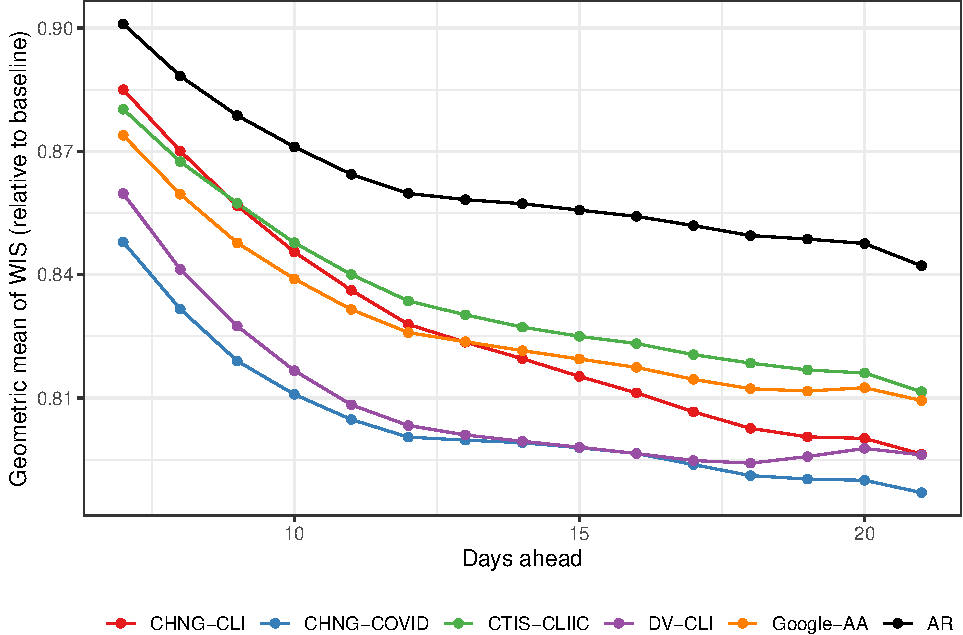
\includegraphics[width=\textwidth]{fig/fcast-alldates-adjusted-1} 

}

\caption{Forcast performance over all periods aggregaged with the geometric mean. Again, the inclusion of data in 2021 leads to improved performance.}\label{fig:fcast-alldates-adjusted}
\end{figure}

\clearpage

\begin{figure}

{\centering 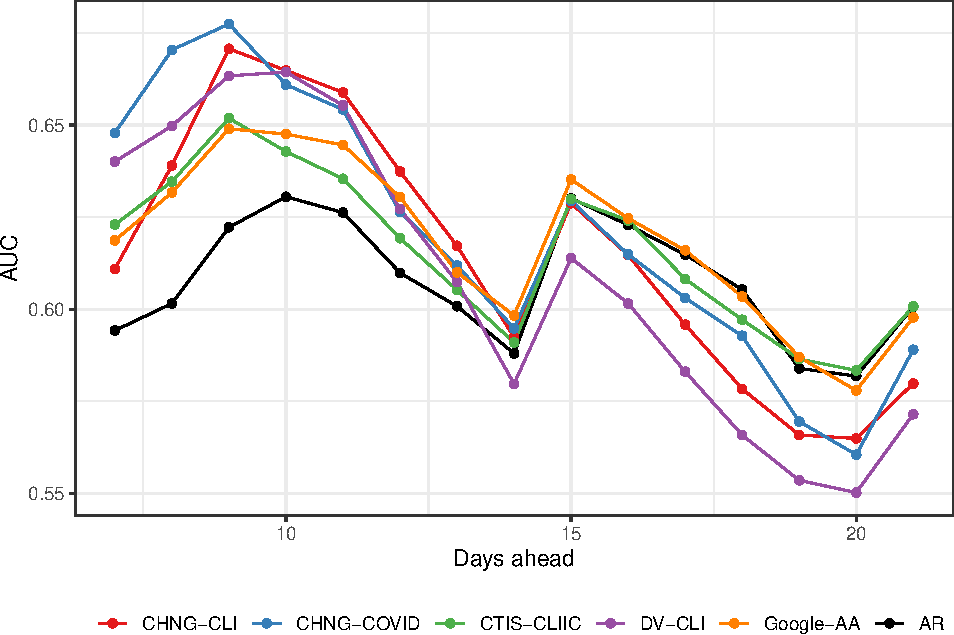
\includegraphics[width=\textwidth]{fig/hot-alldates-1} 

}

\caption{Area under the curve for hotspot predictions including data in 2021. Performance degrades relative to the period in 2020. However, there are far fewer hotspots during this period as case rates declined in much of the country.}\label{fig:hot-alldates}
\end{figure}



%\bibliography{../../common/covidcast.bib,pnas-materials/pnas-sample.bib}



\end{document}
